Mit den Erkenntnissen des vorherigen Kapitels kann sich nun der Konzeption des Hyperaudio-Plugins zugewendet werden. Dabei werden zu Beginn die Zusammenhänge der Komponenten von Hyperaudio-Dokument und Annotationen analysiert und deren Zusammenhänge festgehalten. Diese Zusammenhänge können durch eine Schnittstellendatei abgebildet werden, deren Format in Abschnitt \ref{sec:konfigurationsdatei} definiert wird. Anschließend wird der Datenbankentwurf vorgenommen. Im Anschluss kann sich der Gestaltung der Benutzeroberfläche des Plugins gewidmet werden.


%%%%%%%%%%
\section{Zusammenhänge der Komponenten der Hyperaudio-Anwendung}
Basierend auf der Definition eines Hyperaudio-Dokuments aus Abschnitt \ref{sec:hyperaudio} und der in Abschnitt \ref{sec:anforderungsdefinition} erarbeiteten Anforderungen werden die Zusammenhänge der medialen Komponenten weiter analysiert. Hierbei soll vor allem geklärt werden, wie die einzelnen Komponenten von Hyperaudio-Dokument und Annotationen zusammenhängen und welche Möglichkeiten dadurch gegeben beziehungsweise nicht gegeben sind.


%%%%%%%%%%
\subsection{Komponenten}
Im Mittelpunkt eines Hyperaudio-Dokuments steht eine Audio-Datei. Inhaltlich kann es sich hierbei beispielsweise um einen Vorlesungsvortrag handeln. Man könnte sich auch vorstellen, dass ein Hyperaudio-Dokument aus mehreren aneinandergereihten Audio-Dateien besteht. Dies würde an der grundsätzlichen Problemstellung jedoch nichts ändern und kann im Nachhinein jederzeit als Erweiterung umgesetzt werden. Aus diesem Grund wird in dieser Arbeit nur ein Plugin für ein Hyperaudio-Dokument bestehend aus einer Audio-Datei entwickelt.

Neben dieser zentralen Audio-Datei besteht das Hyperaudio-Dokument aus mehreren Zusatzinhalten, wobei es sich um Bilder, Graphen, Tabellen usw. handeln kann. Entscheidend ist aber, dass diese Zusatzinhalte immer nur eine rein grafische Darstellung verkörpern. Videos mit Ton sind somit beispielsweise nicht als Zusatzinhalt verwendbar, reine Animationen ohne Ton sind aber durchaus möglich.

Als besondere, nämlich externe Komponente, sind die Kommentare zu nennen. Diese gehören nicht zum eigentlichen Hyperaudio-Dokument, sollen aber mit diesem verknüpft werden. Es wird drei verschiedene Arten von Kommentaren geben, nämlich  öffentliche Kommentare, persönliche Notizen und Markierungen. Innerhalb der öffentlichen Kommentare muss noch zwischen den Original-Kommentaren und den Antworten auf diese unterschieden werden. 


%%%%%%%%%%
\subsection{Zusammenhänge}
\label{sec:komponenten_zusammenhänge}
Diese Zusammenhänge der soeben genannten Komponenten sind im UML-Diagramm in Abbildung \ref{fig:UMLAufbau} ersichtlich. Zunächst werden die Zusammenhänge zwischen der Audio-Datei und den Zusatzinhalten betrachtet. Nach dem Master-Slave-Prinzip werden Zusatzinhalte der Audio-Datei untergeordnet. Zu jedem beliebigen Zeitpunkt innerhalb der Abspieldauer der Audio-Datei kann maximal ein Zusatzinhalt gleichzeitig annotiert werden. Es sind also auch Phasen möglich, zu denen keinerlei Zusatzinhalt dargestellt wird. Das Zeitfenster für die Annotation soll mittels einer Start- und Endzeit pro Zusatzinhalt definiert werden, wobei nur die Minuten und Sekunden anzugeben sind. Bei dem Zeitfenster sollte natürlich bedacht werden, dass dieses nicht zu kurz sein sollte. Zwar soll, sobald ein Zusatzinhalt im Player des Hyperaudio-Dokuments angezeigt wird, ein entsprechender \textit{Audio Cue} abgespielt werden, dennoch können bereits einige Sekunden vergehen bis der Studierende seinen Blick dem Player zuwendet.

Auch die Kommentare stehen als externe Komponente in einer gewissen Art und Weise im Zusammenhang mit der Audio-Datei. Dies ergibt sich daraus, dass Kommentare zu einem bestimmten Zeitpunkt innerhalb der Audio-Datei erfasst werden. Während Antworten auf Original-Kommentare erfasst werden können, sind Antworten auf Antworten nicht möglich.

Zwischen Kommentaren und Zusatzinhalten gibt es jedoch keinen direkten Zusammenhang. Solche Zusammenhänge ergeben sich alleine aus den Zeitpunkten der Annotationen. Zusatzinhalte können wiederum in keinem Zusammenhang mit einem anderen Zusatzinhalt stehen.


\begin{figure}[h!]
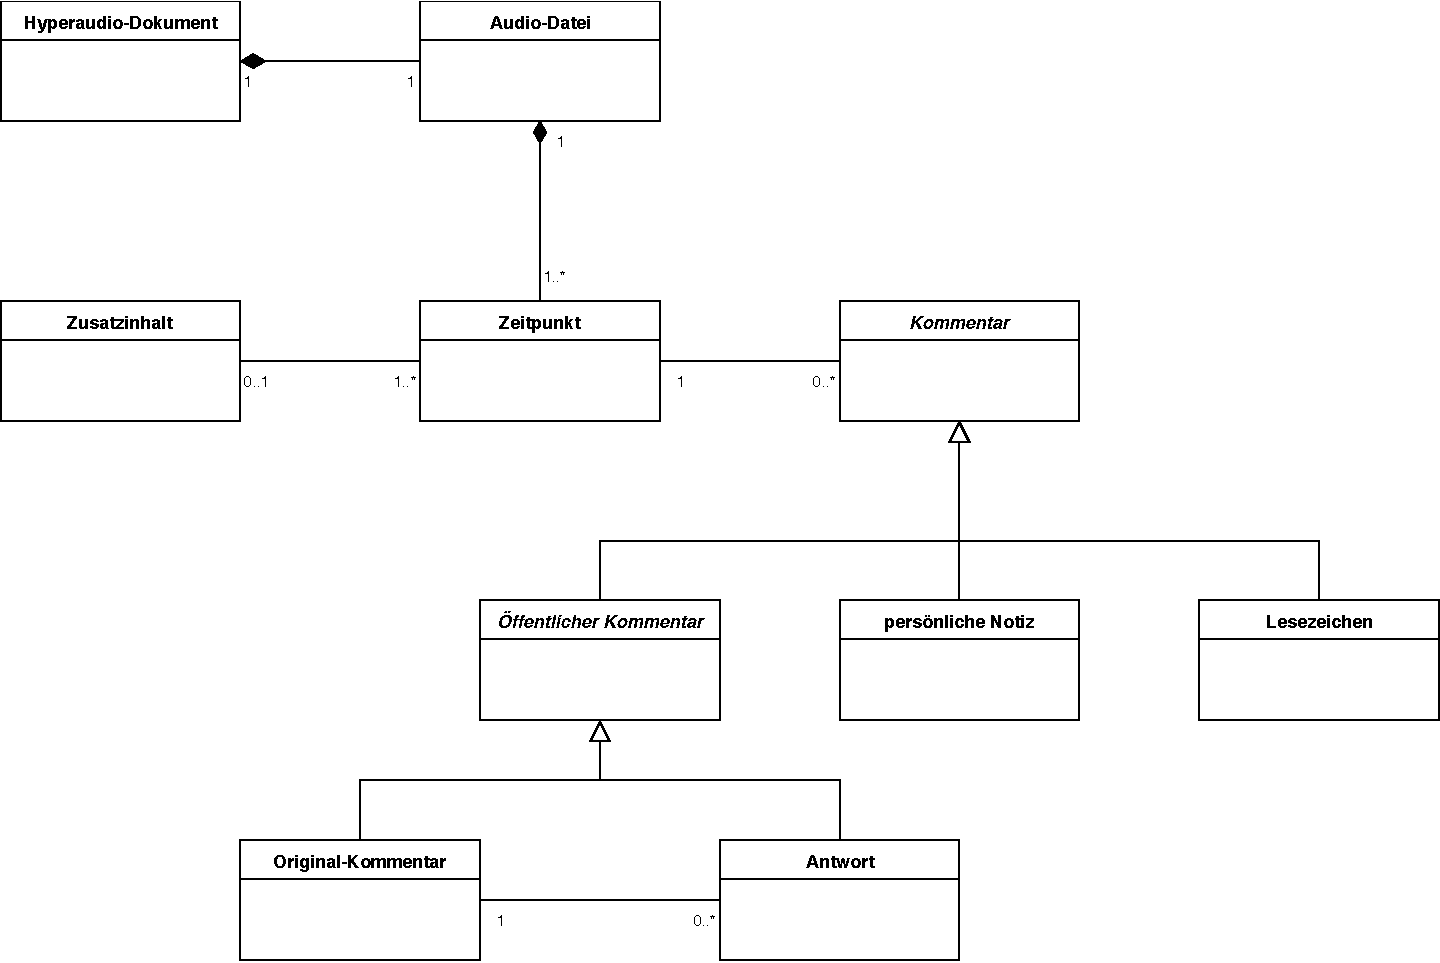
\includegraphics[width=\textwidth,center]{UMLZusammenhaenge.pdf}
\caption{\label{fig:UMLAufbau}Zusammenhänge der Komponenten}
\end{figure}


%%%%%%%%%%
\section{Definition des Schnittstellenformats für Hyperaudio-Dokumente}
\label{sec:konfigurationsdatei}
Um ein Hyperaudio-Dokument zu erstellen, können mehrere Dateien hochgeladen werden. Verpflichtend ist das Bereitstellen einer Audio-Datei. Sollen Zusatzinhalte angezeigt werden, muss neben den Zusatzinhalten selbst auch eine Konfigurationsdatei hochgeladen werden. Darin wird festgehalten, zu welchem Zeitpunkt welcher Zusatzinhalt annotiert werden soll. Darüber hinaus ist es mittels der Konfigurationsdatei möglich Metadaten (Name und Beschreibung des Zusatzinhalts sowie die betroffene Kurseinheit und die zugehörigen Seiten) für die einzelnen Zusatzinhalte anzufügen.
%Wie in der Einleitung dieses Kapitels beschrieben, kann die Konfiguration zu welchem Zeitpunkt welcher Zusatzinhalt annotiert werden soll mittels einer Konfigurationsdatei durchgeführt werden. Diese Vorgehensweise wird nun umgesetzt und die Konfigurationsdatei ist entsprechend zu definieren.
Aufgrund des Einsatzes von PHP und JavaScript innerhalb der Moodle Plugin-Entwicklung bietet sich der Einsatz von JSON (JavaScript Object Notation) an. JSON wird direkt durch JavaScript unterstützt und bietet im Vergleich zu XML (Extensible Markup Language) erhebliche Geschwindigkeitsvorteile \citep{nurseitov2009comparison}.
%JSON is directly supported inside JavaScript [7] and is best suited for JavaScript applications; thus providing significant performance gains over XML, 
Mittels der JSON-Datei sollen folgende Informationen der Zusatzinhalte übertragen werden:

\begin{itemize}
\item Dateiname
\item Name des Zusatzinhaltes
\item Beschreibung des Zusatzinhaltes
\item Kurseinheit
\item Betroffene Seiten innerhalb der Kurseinheit
\item Startzeitpunkt der Annotation
\item Endzeitpunkt der Annotation
\end{itemize}

Entscheidend ist dabei vor allem der Dateiname. Anhand des Dateinamens kann anschließend die Zuordnung der weiteren Informationen zu der entsprechenden Audio-Datei in der Datenbank vorgenommen werden. Eine beispielhaft befüllte Konfigurationsdatei ist in Auflistung \ref{lst:JSON} dargestellt.

\begin{lstlisting}[language=json,
             linewidth=\textwidth,
             caption={Beispielhafte Konfigurationsdatei},
             label={lst:JSON}]             
{
  "additional_contents": {
    "additional_content": [
      {"filename": "Abbildung_1_4.png",
      "name": "Abbildung 1.4",
      "course_unit": 1", 
      "page": "31",
      "description": "Ein kooperativer Editor zur Visualisierung von gemeinsam zu lernenden Vokabeln.",
      "begin": "5",
      "end": "10"},
      {"filename": "Abbildung_1_5.png",
      "name": "Abbildung 1.5",
      "course_unit": "1",
      "page": "32",
      "description": "Verschiedene Komponenten des Papierprototyps.",
      "begin": "15",
      "end": "25"}
    ]
  }
}
\end{lstlisting}
\todo[inline]{JSON Beispieldaten Zeitpunkte korrigieren}
\todo[inline]{JSON-Datei um Autor ergänzen}

%%%%%%%%%%
\section{Datenbankentwurf}
\label{sec:datenbank}
Um die dem Plugin zugrundeliegende Datenbank zu gestalten, wird auf die Erkenntnisse aus Abschnitt \ref{sec:komponenten_zusammenhänge} zurückgegriffen. Das Ergebnis ist dem ER-Diagramm in Abbildung \ref{fig:ERDiagramm} zu entnehmen.

Jede der Datenbanktabellen verfügt über einen Primärschlüssel (\textit{id}). Darüber hinaus wird zu jedem Eintrag gespeichert, wann dieser erstellt (\textit{timecreated}) und zuletzt bearbeitet (\textit{timemodified}) wurde. Für das Abspeichern von Dateien stellt Moodle die Tabelle \textit{files} bereit \citep{moodle2018file}. Dort kann die Datei abgelegt und an anderer Stelle darauf referenziert werden.

Im Mittelpunkt des Hyperaudio-Plugins steht die Tabelle \textit{hyperaudio}. Diese repräsentiert das Hyperaudio-Dokument und die Audio-Datei aus Abbildung \ref{fig:UMLAufbau}. Zunächst wird die ID des Moodle-Kurses (\textit{course}) abgelegt, dem das Hyperaudio-Dokument zugeordnet ist. Während die Audio-Datei selbst in der bereits erwähnten Tabelle \textit{files} zu finden ist, wird in der Tabelle \textit{hyperaudio} deren Dateiname (\textit{audiofile}) festgehalten. Zum Hyperaudio-Dokument können außerdem Name und Ersteller in den Spalten \textit{name} und \textit{author} hinterlegt werden. Eine optionale Beschreibung kann entsprechend dem de-facto-Standard der Moodle-Plugin-Entwicklung über \textit{introformat} und \textit{intro} hinzugefügt werden \citep{moodle2016activity}.

Bei der Tabelle \textit{hyperaudio\underline{{ }}config} handelt es sich um eine Tabelle, in welcher die in Abschnitt \ref{sec:konfigurationsdatei} beschriebene Konfigurationsdatei gespeichert wird (\textit{file} enthält den Dateinamen als Referenz auf die \textit{files}-Tabelle). Daneben wird nur noch der Fremdschlüssel \textit{hyperaudio\underline{{ }}id} auf die Tabelle \textit{hyperaudio} als Zuordnung zum Hyperaudio-Dokument benötigt.

Zur Ablage der annotierten Zusatzinhalte dient die Tabelle \textit{additional\underline{{ }}content}. Auch hier steht der Name der Datei in der Spalte \textit{file} als Referenz auf die \textit{files}-Tabelle. Ebenso dient der Fremdschlüssel \textit{hyperaudio\underline{{ }}id} zur Verknüpfung des Zusatzinhalts mit der Audio-Datei. Des Weiteren werden folgende Metainformationen zum Zusatzinhalt abgespeichert:

\begin{itemize}

\item Name des Zusatzinhalts (\textit{name})
\item optional: Beschreibung (\textit{description})
\item optional: Kurseinheit (\textit{course\underline{{ }}unit})
\item optional: Seitenangabe (\textit{page})
\item Startzeitpunkt der Annotation innerhalb des Hyperaudio-Dokuments (\textit{begin})
\item Endzeitpunkt der Annotation innerhalb des Hyperaudio-Dokuments (\textit{end})

\end{itemize}

Die Tabelle \textit{hyperaudio\underline{{ }}comments} dient der Speicherung der vier in Abbildung \ref{fig:UMLAufbau} modellierten Kommentararten. Der Zusammenhang zum Hyperaudio-Dokument wird analog per Fremdschlüssel \textit{hyperaudio\underline{{ }}id} hergestellt. Neben dem textuellen Kommentar (\textit{commenttext}), werden auch der Verfasser in Form der \textit{userid}, die Art des Kommentars (\textit{comment\underline{{ }}type}\footnote{\texttt{COMMENT}, \texttt{NOTE} oder \texttt{MARK}}) und der Annotationszeitpunkt (\textit{timeannotated}) gespeichert. Für den Fall, dass es sich um einen Antwortkommentar handelt, wird in der Spalte \textit{comment\underline{{ }}id} die Referenz auf den Original-Kommentar festgehalten.

\begin{figure}[h!]
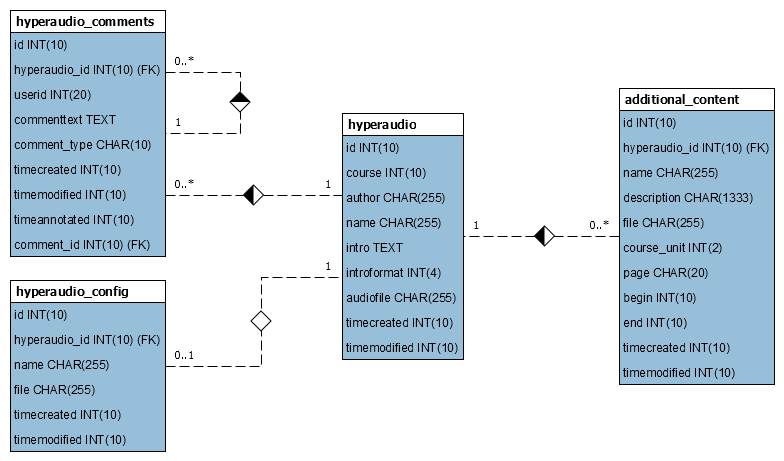
\includegraphics[width=\textwidth,center]{ERDiagramm.png}
\caption{\label{fig:ERDiagramm}ER-Diagramm der Datenbank des Moodle-Plugins}
\end{figure}


%%%%%%%%%%
\section{Gestaltung der Benutzeroberfläche}
Damit den Lehrenden und Studierenden die im vorherigen Abschnitt beschriebenen Nutzungsszenarien möglichst leicht fallen, wenden wir uns nun der Gestaltung der Benutzeroberfläche zu. \glqq Das Design der Benutzeroberfläche stellt einen zentralen Aspekt für die Gebrauchstauglichkeit eines Softwareprodukts dar\grqq{} \citep[S. 1]{oppermann2002user}. Einen dementsprechend hohen Stellenwert wollen wir der Benutzeroberfläche unseres Moodle-Plugins zuschreiben. Bei der Gestaltung der Benutzeroberfäche gehen wir wie bereits bei der Analyse in Kapitel \ref{cha:analyse} vor und teilen die Benutzeroberfläche in Teilbereiche auf. Im ersten Schritt betrachten wir zunächst die Seite eines Hyperaudio-Dokuments innerhalb eines Kurses. Danach widmen wir uns der Administrationsseite eines Hyperaudio-Dokuments innerhalb eines Kurses. Im letzten Schritt wenden wir uns den verschiedenen Integrationsmöglichkeiten innerhalb der allgemeinen Moodle-Oberfläche zu.

Generell erfolgen alle Entscheidungen bezüglich der Oberfläche auf Basis von Skizzen. Diese wurden mittels des Programms \textit{Balsamiq Mockups 3.5.15}\footnote{https://balsamiq.com/} erstellt. Anhand der Skizzen können Vor- und Nachteile der verschiedenen Designansätze schnell erkannt und auf Grund dessen sachliche Entscheidungen getroffen werden. 
%Durch das Arbeiten mit Skizzen erkennt man schneller welche Vor- und Nachteile die verschiedenen Designansätze bieten und kann auf Grund dessen dann sachliche Entscheidungen treffen.


%%%%%%%%%%
%\subsection{Seite eines Hyperaudio-Dokuments}
Die Seite eines Hyperaudio-Dokuments lässt sich grob, wie bereits in Abbildung \ref{fig:MockupBereiche} dargestellt, in die Bereiche Player, Galerie und Kommentarsektion aufteilen. Wir werden nun zunächst für jeden dieser Bereiche verschiedene Designs diskutieren und uns dann für eines entscheiden. Danach erfolgt die Entscheidung über die Anordnung dieser Bereiche auf der Seite eines Hyperaudio-Dokuments.


%%%%%%%%%%
\subsubsection{Player}
Beim Player für Hyperaudio-Dokumente müssen, neben den üblichen Mediensteuerungselementen, gleich mehrere zusätzliche Elemente visualisiert werden. Zum einen müssen zu den entsprechenden Zeitpunkten die annotierten Zusatzinhalte dargestellt werden. Auf der anderen Seiten sollen auch die annotierten öffentlichen Kommentare, persönlichen Notizen und Markierungen veranschaulicht werden. Dem Wunsch, direkt über den Player öffentliche Kommentare, persönlichen Notizen und Markierungen erstellen und in letzterem Fall sogar löschen zu können, muss auch Sorge getragen werden.

Der Player für Hyperaudio-Dokumente wird, wie in Abbildung \ref{fig:MockupPlayerVersion1} zusehen ist, als Videoplayer umgesetzt. Somit werden die Zusatzinhalte an Stelle eines Videos dargestellt. Die persönlichen Notizen und Markierungen werden innerhalb der Abspielleiste mittels unterschiedlich gefärbter Kreisen illustriert. In diesem Fall sollen die roten Kreise Markierungen und der blaue Kreis eine persönliche Notiz widerspiegeln. Unterhalb der Mediensteuerung ist ein Bereich zu finden, in dem die Kommentare grafisch sichtbar gemacht werden sollen. Hierfür wird jedes Hyperaudio-Dokument in die gleiche fixe Anzahl an Zeitfenstern aufgeteilt. Diese Zeitfenster werden durch senkrecht orientierte Balken dargestellt, deren Höhe für die Anzahl der zu diesem Zeitfenster erfassten Kommentare stehen soll. Unter dem Bereich für die Kommentare befindet sich eine Eingabemaske, mit welcher öffentliche Kommentare und persönliche Notizen erfasst werden können. Das Erstellen und Löschen von Markierungen soll mittels Rechtsklick auf die entsprechende Stelle innerhalb der Abspielleiste in einem dazugehörigen Kontextmenü umgesetzt werden. Dies ist in Abbildung \ref{fig:MockupPlayerVersion1} mittels der beiden Mauszeiger, den Pfeilen und den entsprechenden Buttons symbolisiert.

\todo[inline]{Unterscheidung nicht nur durch Farbe (Barrierefreiheit)}

%\begin{figure}[h!]
%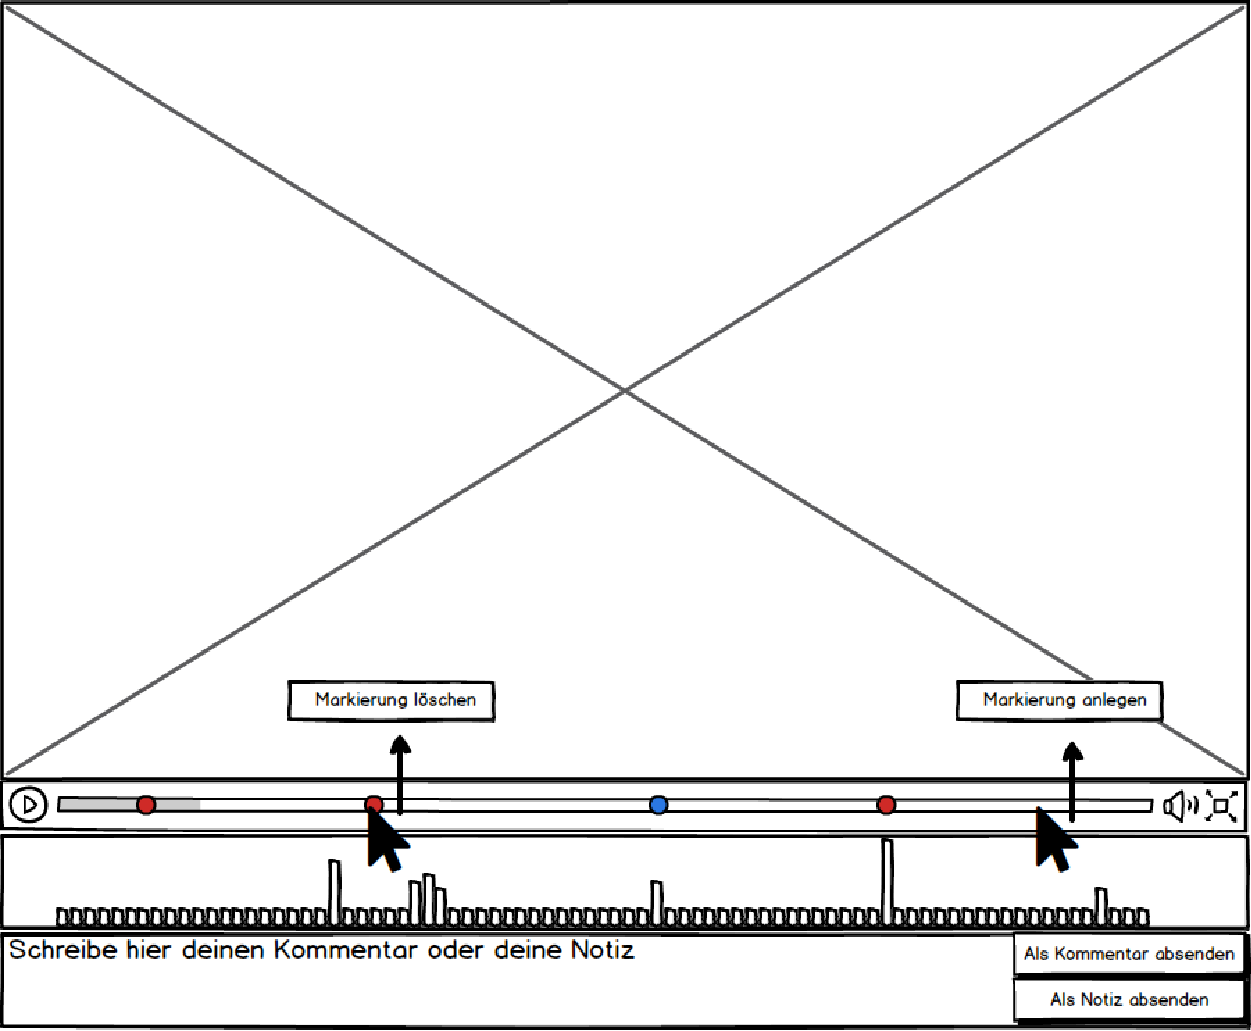
\includegraphics[width=0.8\textwidth,center]{MockupPlayerVersion1.pdf}
%\caption{\label{fig:MockupPlayerVersion1} Erster Entwurf des Players}
%\end{figure}

In einer zweiten Variante des Players wird die Visualisierung der persönlichen Notizen von der Abspielleiste in den Bereich der Kommentare verschoben. Wie in Abbildung \ref{fig:MockupPlayerVersion2} ersichtlich,  wird der Balken für den Zeitraum, in dem die persönlichen Notiz liegt, zu einem gewissen Teil blau eingefärbt. Dadurch wird nebenbei das Handling der Punkte in der Abspielleiste vereinheitlicht, da es hier nur noch die Markierungen mit Interaktionsmöglichkeit gibt.

\begin{figure}[h!]
\begin{subfigure}[c]{\textwidth}
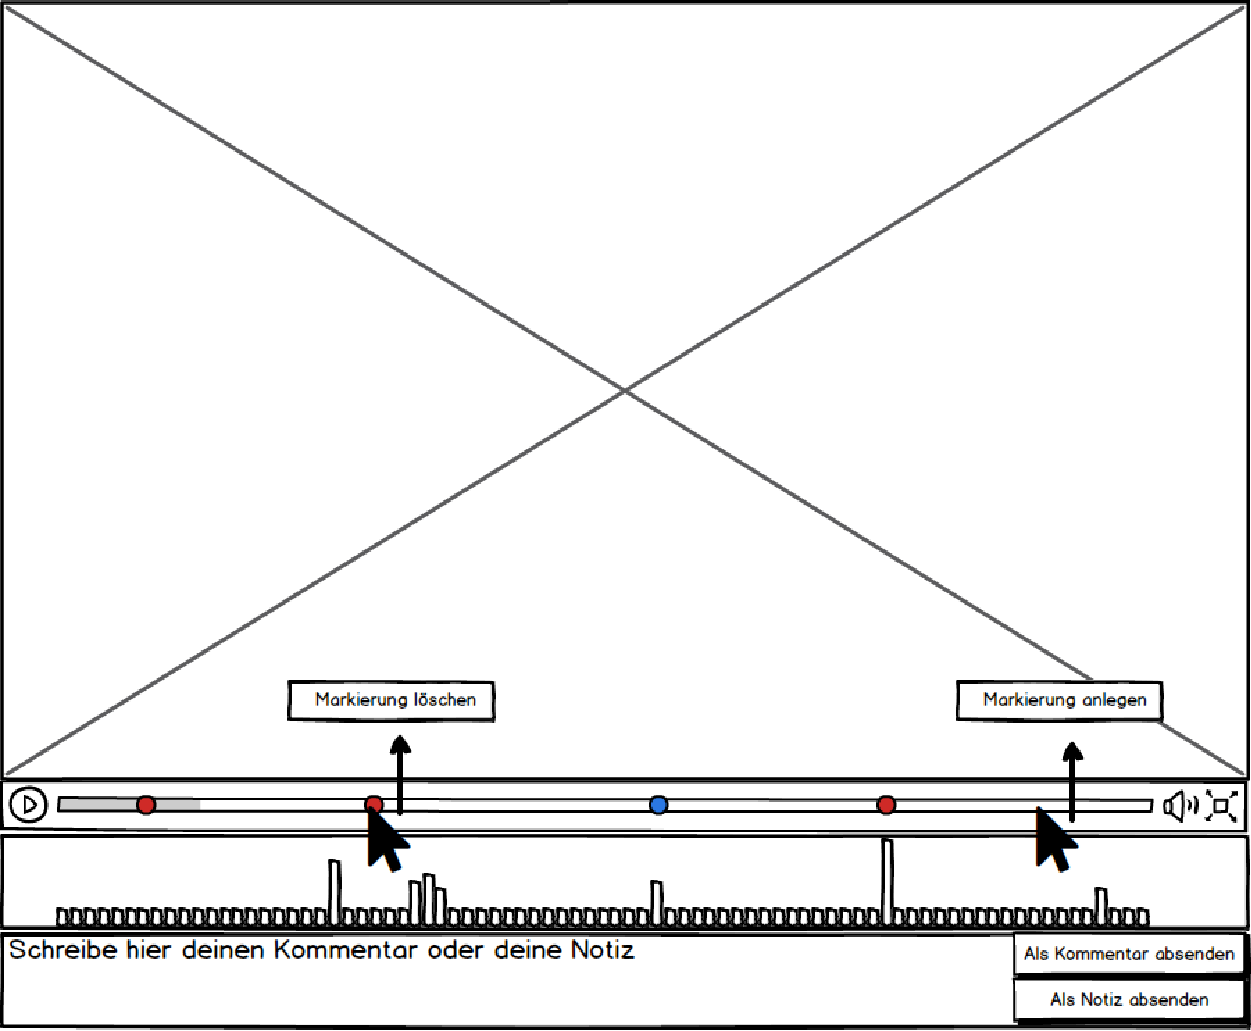
\includegraphics[width=0.8\textwidth,center]{MockupPlayerVersion1.pdf}
\subcaption{Erste Version}
\label{fig:MockupPlayerVersion1}
\end{subfigure}
\par\bigskip
\begin{subfigure}[c]{\textwidth}
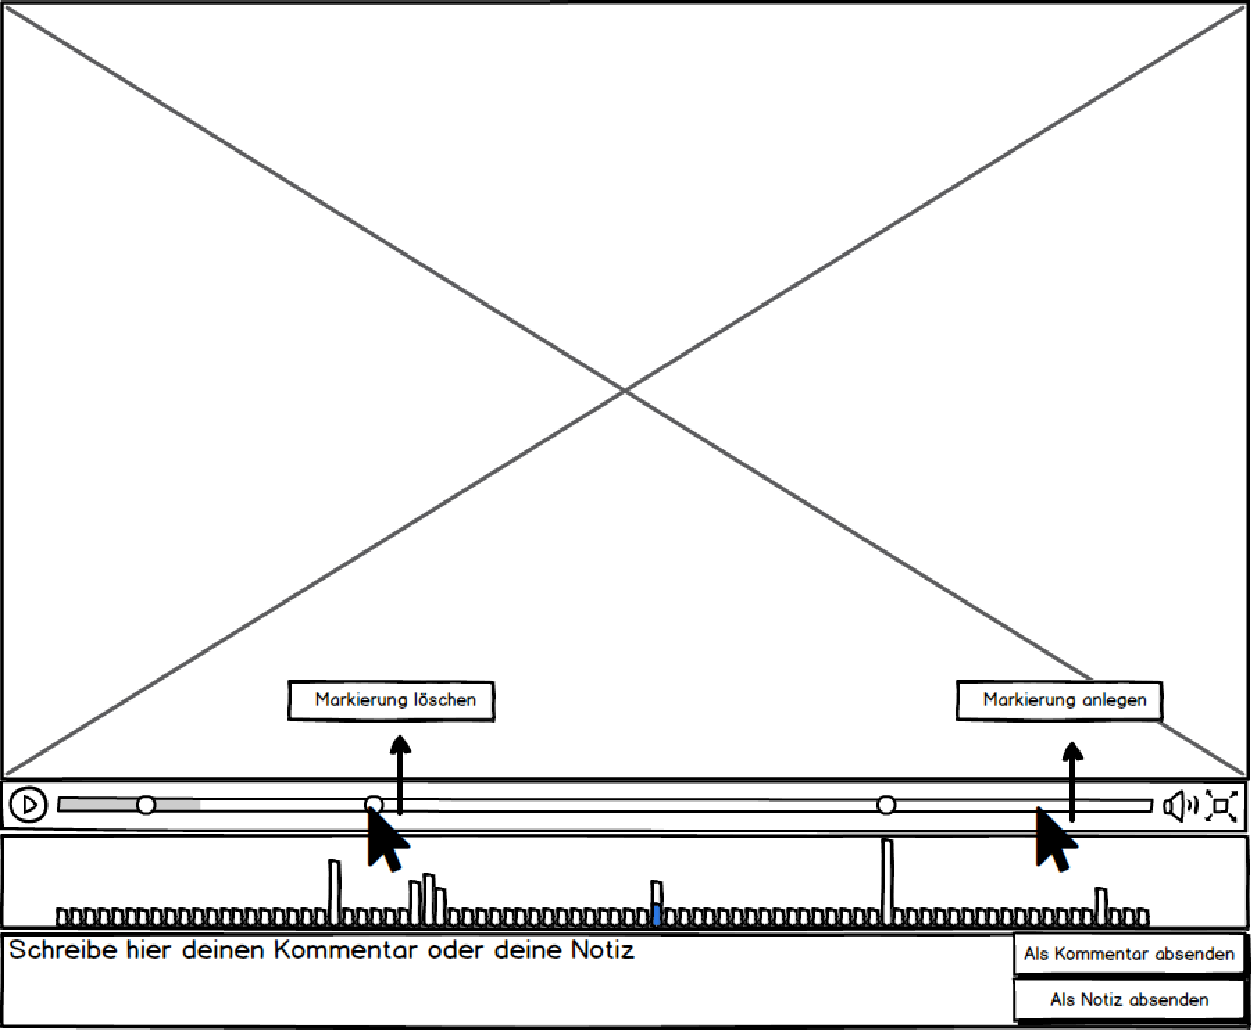
\includegraphics[width=0.8\textwidth,center]{MockupPlayerVersion2.pdf}
\subcaption{Finale Version}
\label{fig:MockupPlayerVersion2}
\end{subfigure}
\caption{Benutzeroberfläche - Player}
\label{fig:MockupPlayerVersion}
\end{figure}

%\begin{figure}[h!]
%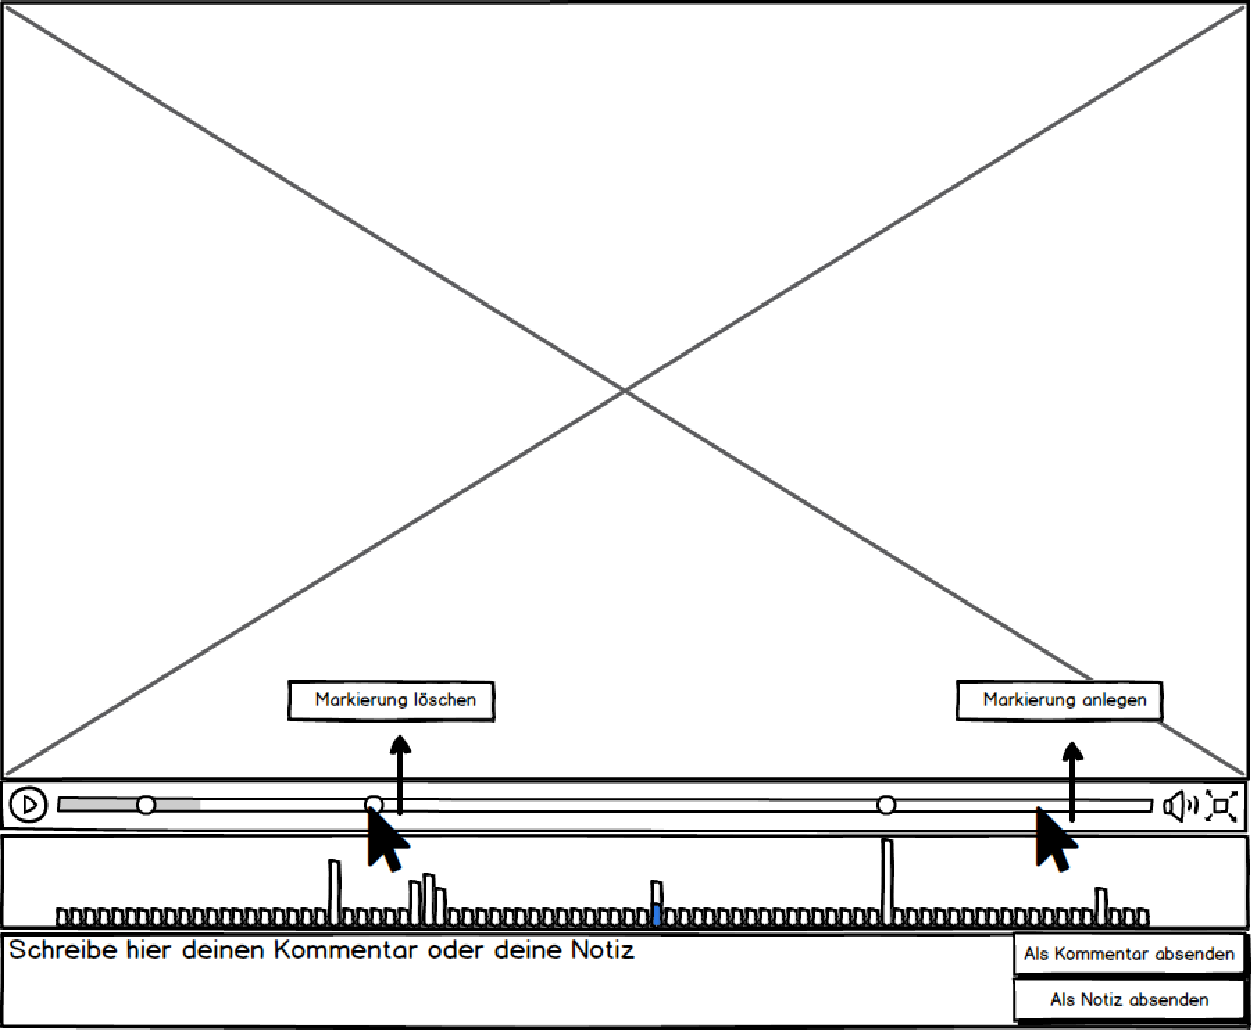
\includegraphics[width=.8\textwidth,center]{MockupPlayerVersion2.pdf}
%\caption{\label{fig:MockupPlayerVersion22}Zweiter Entwurf des Players}
%\end{figure}


%%%%%%%%%%
\subsubsection{Galerie}
Die Galerie soll dazu dienen, einen Überblick über die vorhanden Zusatzinhalte zu bieten. Die Zusatzinhalte stellen alle einen grafischen Inhalt dar. Dementsprechend kann jeder Zusatzinhalt durch ein kleines Vorschaubild repräsentiert werden. 
Eine weitere Grundfunktionalität einer Galerie ist die vergrößerte Anzeige der in der Vorschau dargestellten Inhalte, die auch in unserer Galerie zur Verfügung stehen soll. Beim Erstellen des Designs muss zusätzlich auch die Anforderung der Rückkopplung zum Player bedacht werden (siehe Abschnitt \ref{sub:AnforderungenOberflaeche}). 
%Neben der Grundfunktionalität einer Galerie, dass der ausgewählte Zusatzinhalt vergrößert angezeigt werden können soll, muss beim Erstellen des Designs auch die Anforderung der Rückkopplung zum Player bedacht werden (siehe Abschnitt \ref{sub:AnforderungenOberflaeche}). 

Die einfachste Umsetzung der Galerie ist eine Darstellung der Zusatzinhalte in einem einfachen Grid  mit Scrollbalken, wie es in Abbildung \ref{fig:MockupGalerieGrid} zu sehen ist. Zusätzlich wird das Grid um zwei Buttons für eine vergrößerte Ansicht des Zusatzinhalts sowie für die Rückkopplung zum Player ergänzt. Um eine dieser beiden Aktionen auszuführen, müsste also der gewünschte Zusatzinhalt markiert und der entsprechende Button betätigt werden.

%\begin{figure}[h!]
%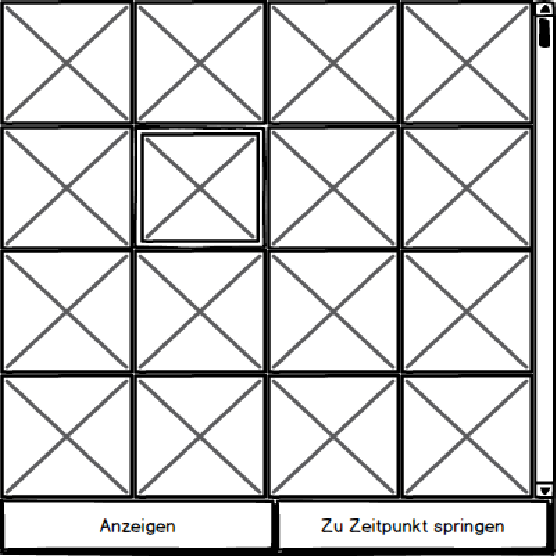
\includegraphics[width=.5\textwidth,center]{MockupGalerieGrid.pdf}
%\caption{\label{fig:MockupGalerieGrid}Garlerie als einfaches Grid}
%\end{figure}

Diese Variante hat den Vorteil, dass besonders viele Zusatzinhalte gleichzeitig angezeigt werden können. Auf der anderen Seite erhalten wir aber keinerlei Informationen zu den Zusatzinhalten. In der zweiten Variante, bei dem das Grid um einen Bereich für Details ergänzt wurde, kann man zumindest die Details des ausgewählten Zusatzinhaltes einsehen. Diese in Abbildung \ref{fig:MockupGalerieGridErweitert} erkennbaren Details sind natürlich von den vorhandenen Metadaten abhängig. Nachteil ist in diesem Fall aber, dass, durch den Bereich für die Details, bei gleicher Größe der Galerie weniger Zusatzinhalte zur selben Zeit dargestellt werden können. Das führt dazu, dass die Verwendung des Scrollbalkens häufiger notwendig wird.

%\begin{figure}[h!]
%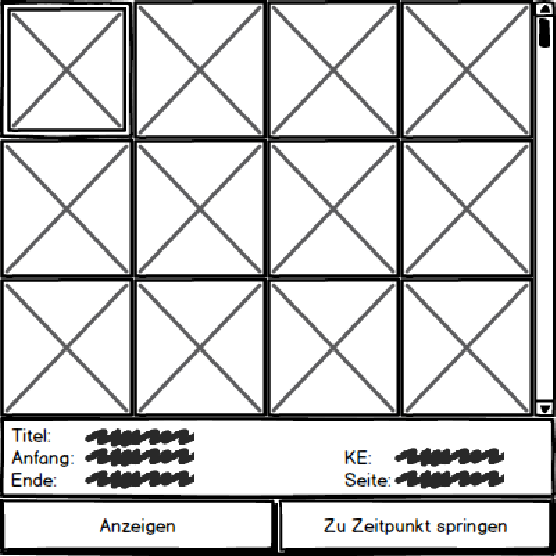
\includegraphics[width=.5\textwidth,center]{MockupGalerieGridErweitert.pdf}
%\caption{\label{fig:MockupGalerieGridErweitert}Galerie als Grid mit Bereich für Details}
%\end{figure}

Bei einer Darstellung der Zusatzinhalte als Kacheln, wie in Abbildung \ref{fig:MockupGalerieKacheln} zu sehen, können gleichzeitig für alle vorhandenen Zusatzinhalte die Details angezeigt werden. Durch diese Art der Darstellung passen jedoch noch weniger Zusatzinhalte auf die gleiche Fläche.

%\begin{figure}[h!]
%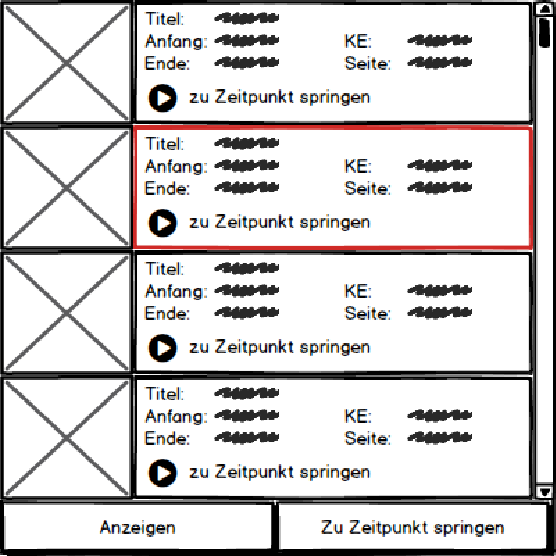
\includegraphics[width=.5\textwidth,center]{MockupGalerieKacheln.pdf}
%\caption{\label{fig:MockupGalerieKacheln}Galerie mit Darstellung in Kachelform}
%\end{figure}

Eine besonders schicke Art der Darstellung wäre die des Cover Flows, bekannt aus verschiedenen Musikplayern. In Abbildung \ref{fig:MockupGalerieCoverFlow} ist zu erkennen, dass auch hier ausschließlich Details des aktuell ausgewählten Zusatzinhaltes sichtbar sind. Des Weiteren hat diese Darstellungsweise den großen Nachteil, dass auch nicht auf einen Blick alle verfügbaren Zusatzinhalte ersichtlich sind. Dies erschwert das Durchsuchen der Zusatzinhalte ungemein. Somit ist diese Art der Darstellung zwar schön anzusehen, aber nicht sonderlich gebrauchstauglich im Zusammenhang dieser Arbeit.

%\begin{figure}[h!]
%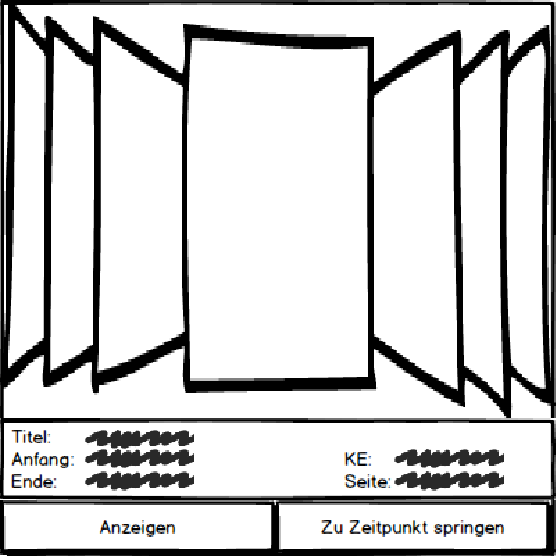
\includegraphics[width=.5\textwidth,center]{MockupGalerieCoverFlow.pdf}
%\caption{\label{fig:MockupGalerieCoverFlow}Galerie als Cover Flow}
%\end{figure}

Letztlich stellt sich die optimierte Variante der Kachel Darstellung aus Abbildung \ref{fig:MockupGalerieFinal} als beste Lösung heraus. Die Optimierung besteht daraus, dass die beiden Buttons obsolet gemacht werden. Dies kann zum einen erreicht werden, indem die vergrößerte Darstellung durch einen Klick auf die Abbildung des Zusatzinhaltes ausgelöst wird. Zum anderen bietet der Bereich der Details noch ausreichend Platz, um hier die Funktion zur Rückkopplung an den Player einzufügen. Durch diese Verbesserungen wird nicht nur mehr Platz geschaffen, sondern auch die Benutzerfreundlichkeit erhöht, indem der Vorgang zum Anzeigen der vergrößerten Ansicht beziehungsweise des Springens an den entsprechenden Zeitpunkt jeweils um einen Klick reduziert wurde.

\begin{figure}[h!]
\begin{subfigure}[c]{0.5\textwidth}
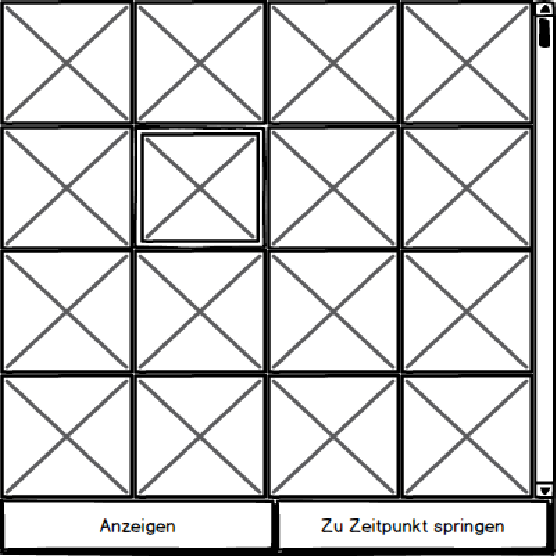
\includegraphics[width=0.8\textwidth,center]{MockupGalerieGrid.pdf}
\subcaption{Galerie als einfaches Grid}
\label{fig:MockupGalerieGrid}
\end{subfigure}%
\begin{subfigure}[c]{0.5\textwidth}
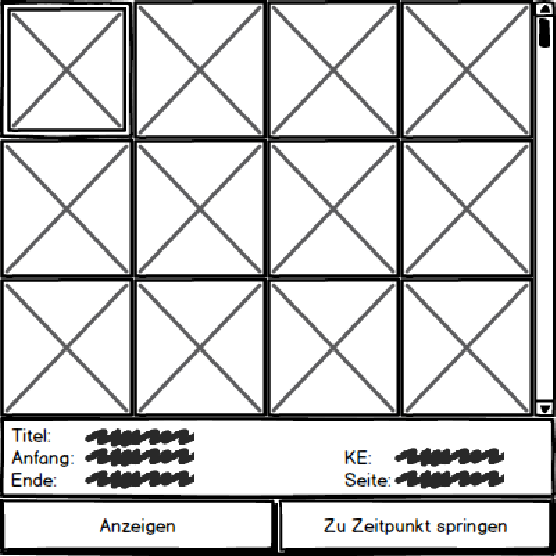
\includegraphics[width=0.8\textwidth,center]{MockupGalerieGridErweitert.pdf}
\subcaption{Galerie als Grid mit Bereich für Details}
\label{fig:MockupGalerieGridErweitert}
\end{subfigure}
\par\bigskip
\begin{subfigure}[c]{0.5\textwidth}
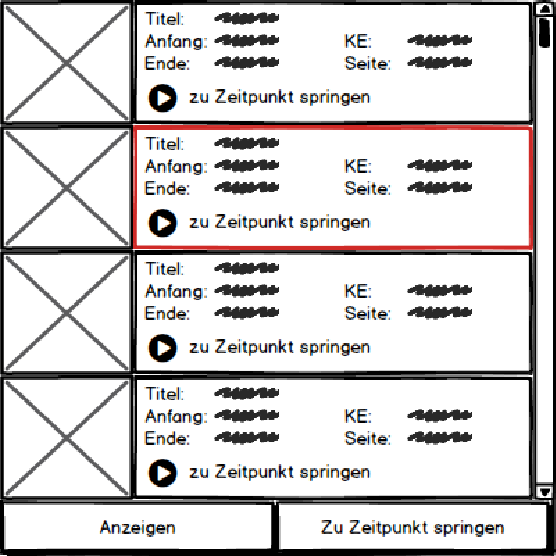
\includegraphics[width=0.8\textwidth,center]{MockupGalerieKacheln.pdf}
\subcaption{Galerie mit Darstellung in Kachelform}
\label{fig:MockupGalerieKacheln}
\end{subfigure}%
\begin{subfigure}[c]{0.5\textwidth}
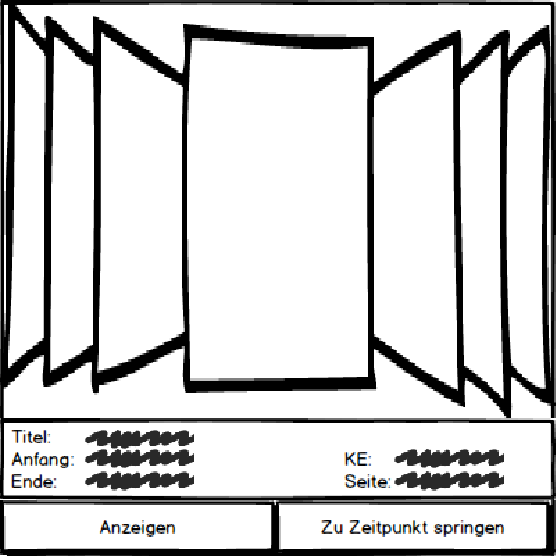
\includegraphics[width=0.8\textwidth,center]{MockupGalerieCoverFlow.pdf}
\subcaption{Galerie als Cover Flow}
\label{fig:MockupGalerieCoverFlow}
\end{subfigure}
\par\bigskip
\begin{subfigure}[c]{\textwidth}
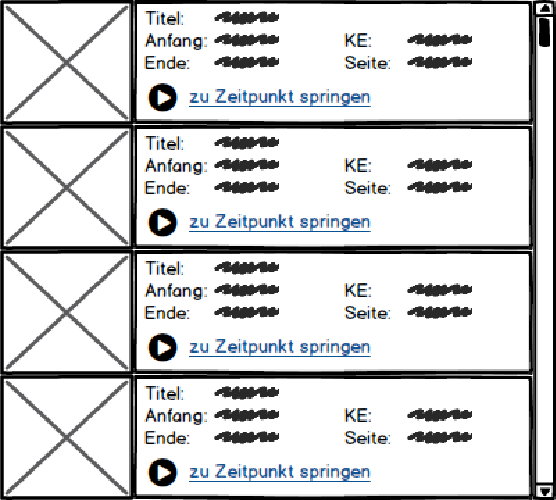
\includegraphics[width=0.4\textwidth,center]{MockupGalerieFinal.pdf}
\subcaption{Finale Version der Galerie}
\label{fig:MockupGalerieFinal}
\end{subfigure}
\caption{Benutzeroberfläche - Galerie}
\label{fig:MockupGalerie}
\end{figure}


%\begin{figure}[h!]
%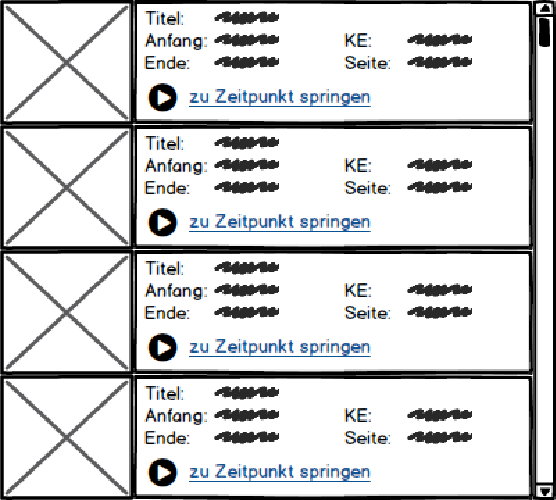
\includegraphics[width=.5\textwidth,center]{MockupGalerieFinal.pdf}
%\caption{\label{fig:MockupGalerieFinal}Finale Version der Galerie}
%\end{figure}

%%%%%%%%%%
\subsubsection{Kommentarsektion}
Die Kommentarsektion ist für die Anzeige der öffentlichen Kommentare sowie der persönlichen Notizen zuständig. Zusätzlich muss eine Suchmaske auf Basis der Anforderungen aus Abschnitt \ref{sub:AnforderungenKommentarsektion} in die Oberfläche integriert werden.

Abbildung \ref{fig:MockupKommentarsektionVersion1} zeigt eine erste Version der Kommentarsektion. Neben der Suchmaske im Kopfbereich befinden sich zwei Checkboxen. Diese ermöglichen es dem Betrachter nach öffentlichen Kommentaren und persönlichen Notizen zu filtern. Im benachbarten Dropdown-Menü kann die Grundlage der Sortierung bestimmt werden. Die Sortierung kann nach Erstellungsdatum beziehungsweise nach Zeitpunkt der Annotation innerhalb des Hyperaudio-Dokuments erfolgen. Unterhalb dieser Funktionen befindet sich die Anzeige der Kommentare und Notizen. Sowohl bei Kommentaren als auch bei Notizen wird neben dem Erstellungsdatum auch der Annotationszeitpunkt festgehalten. Dieser wird als Link umgesetzt, sodass bei einem Klick die Rückkopplung an den Player erfolgen kann. Bei Kommentaren gibt es nach Betätigung der \textit{Antworten}-Schaltfläche noch eine zusätzliche Eingabemaske zum Verfassen von Antworten. Persönliche Notizen werden durch ein Schloss-Symbol hinter dem Erstellungsdatum visualisiert. Zusätzlich befinden sich noch jeweils zwei Buttons zum Bearbeiten und Löschen auf der rechten Seite einer Notiz.

%\begin{figure}[h!]
%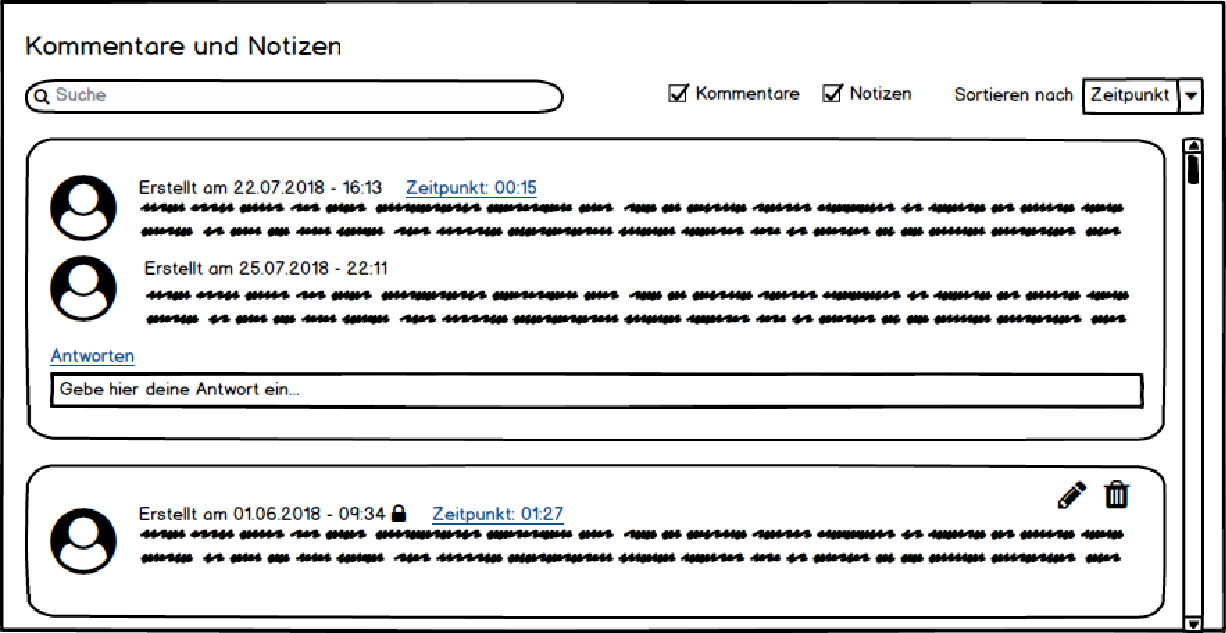
\includegraphics[width=\textwidth,center]{MockupKommentarsektionVersion1.pdf}
%\caption{\label{fig:MockupKommentarsektionVersion1}Erste Version der Kommentarsektion}
%\end{figure}

Im nochmals verbesserten Design der Kommentarsektion, welches in Abbildung \ref{fig:MockupKommentarsektionFinal} abgebildet ist, werden die Antworten auf Kommentare eingerückt dargestellt. Diese Darstellung führt zu einer besseren Übersichtlichkeit und ist auch aus anderen modernen Anwendungen bekannt.

\begin{figure}[h!]
\begin{subfigure}[c]{\textwidth}
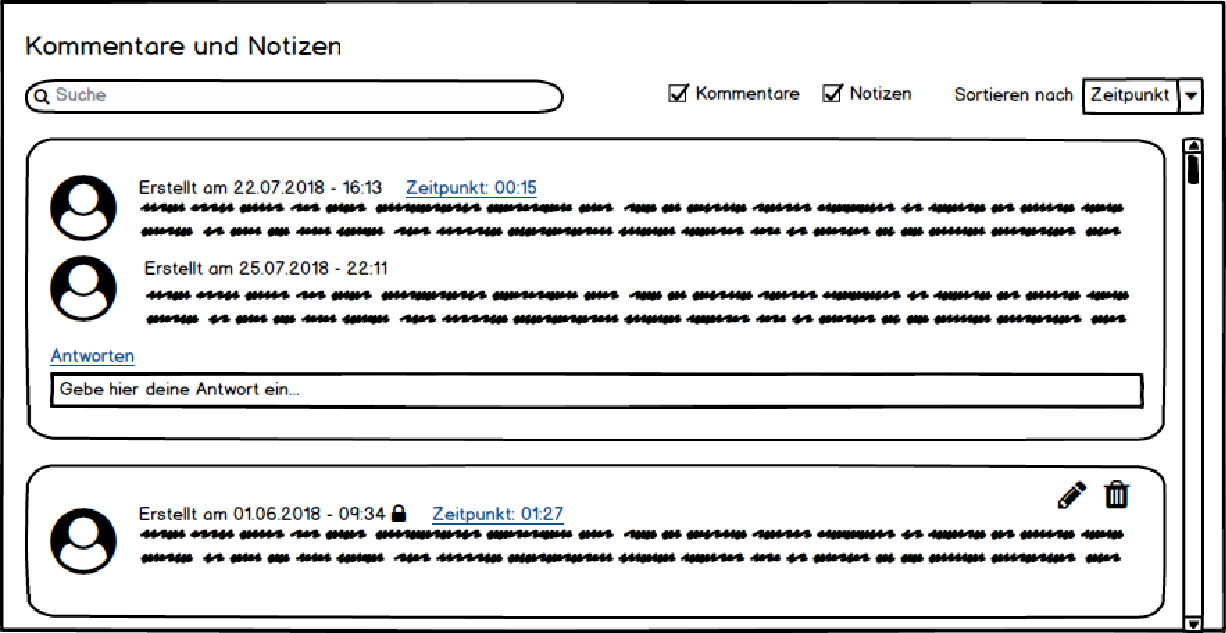
\includegraphics[width=\textwidth,center]{MockupKommentarsektionVersion1.pdf}
\subcaption{Erste Version}
\label{fig:MockupKommentarsektionVersion1}
\end{subfigure}
\par\bigskip
\begin{subfigure}[c]{\textwidth}
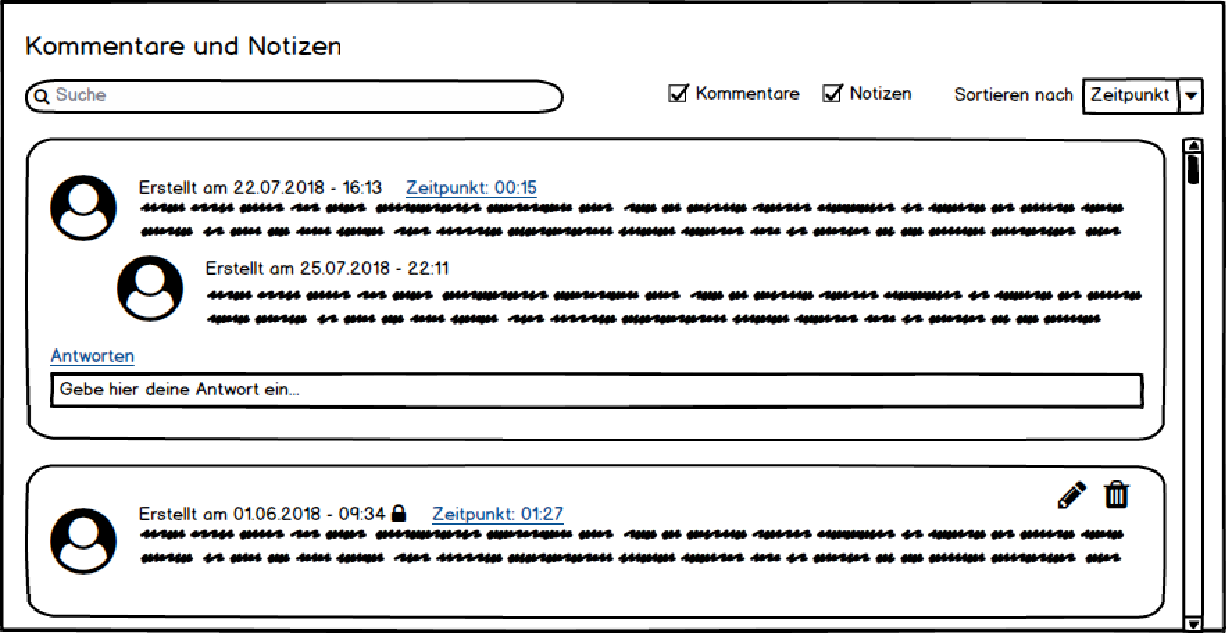
\includegraphics[width=\textwidth,center]{MockupKommentarsektionFinal.pdf}
\subcaption{Finale Version}
\label{fig:MockupKommentarsektionFinal}
\end{subfigure}
\caption{Benutzeroberfläche - Kommentarsektion}
\label{fig:MockupKommentarsektion}
\end{figure}

%\begin{figure}[h!]
%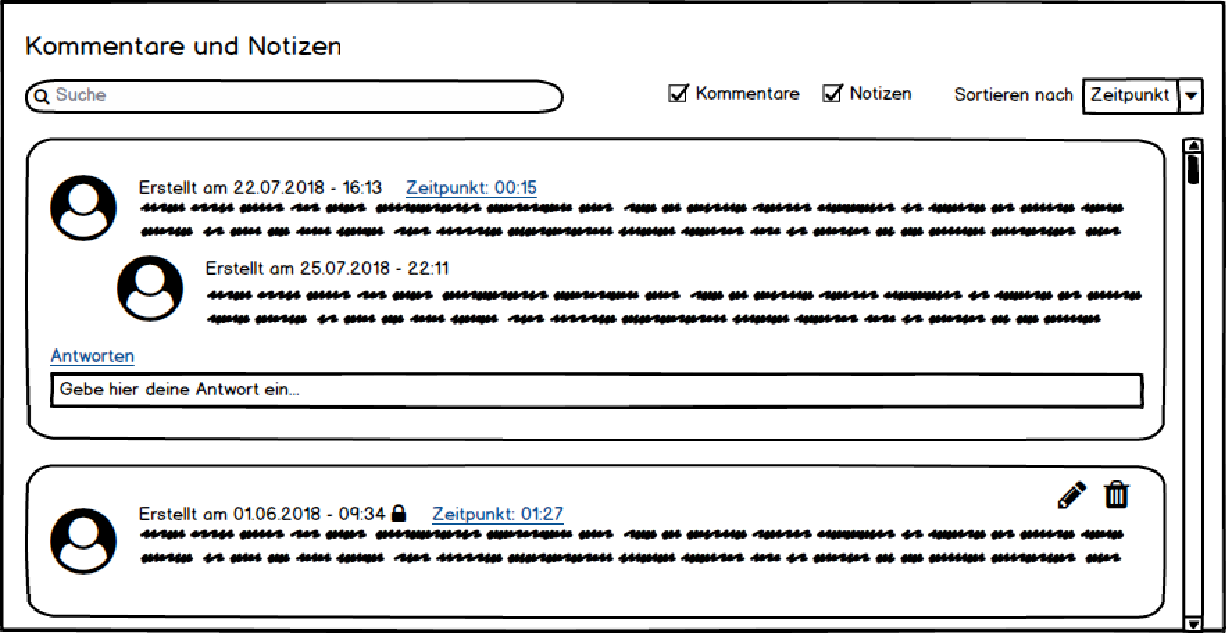
\includegraphics[width=\textwidth,center]{MockupKommentarsektionFinal.pdf}
%\caption{\label{fig:MockupKommentarsektionFinal}Finale Version der Kommentarsektion}
%\end{figure}


%%%%%%%%%%
\subsubsection{Zusammenführen der Elemente}
Im ersten Schritt führen wir die jeweils favorisierten Elemente in ein Layout zusammen. Dabei orientieren wir uns zunächst an unserer grobe Skizze aus Kapitel \ref{cha:analyse}. Wie nun in Abbildung \ref{fig:MockupSeiteLayoutVersion1} zu erkennen ist, ist die Kommentarsektion so in die Breite gezogen, dass das Lesen der Inhalte unangenehm werden kann. Aus diesem Grund wird in der finalen Version (siehe Abbildung \ref{fig:MockupSeiteLayoutFinal}) die Breite der Kommentarsektion auf die Breite des Players beschränkt. Dies hat zeitgleich zur Folge, dass der nun vorhandene freie Platz für die Galerie verwendet werden kann. Spätestens hiermit wird der Nachteil der gewählten Darstellungsweise der Galerie egalisiert, da nun ausreichend viele Zusatzinhalte ohne die Verwendung des Scrollbalkens eingesehen werden können.

%\begin{figure}[h!]
%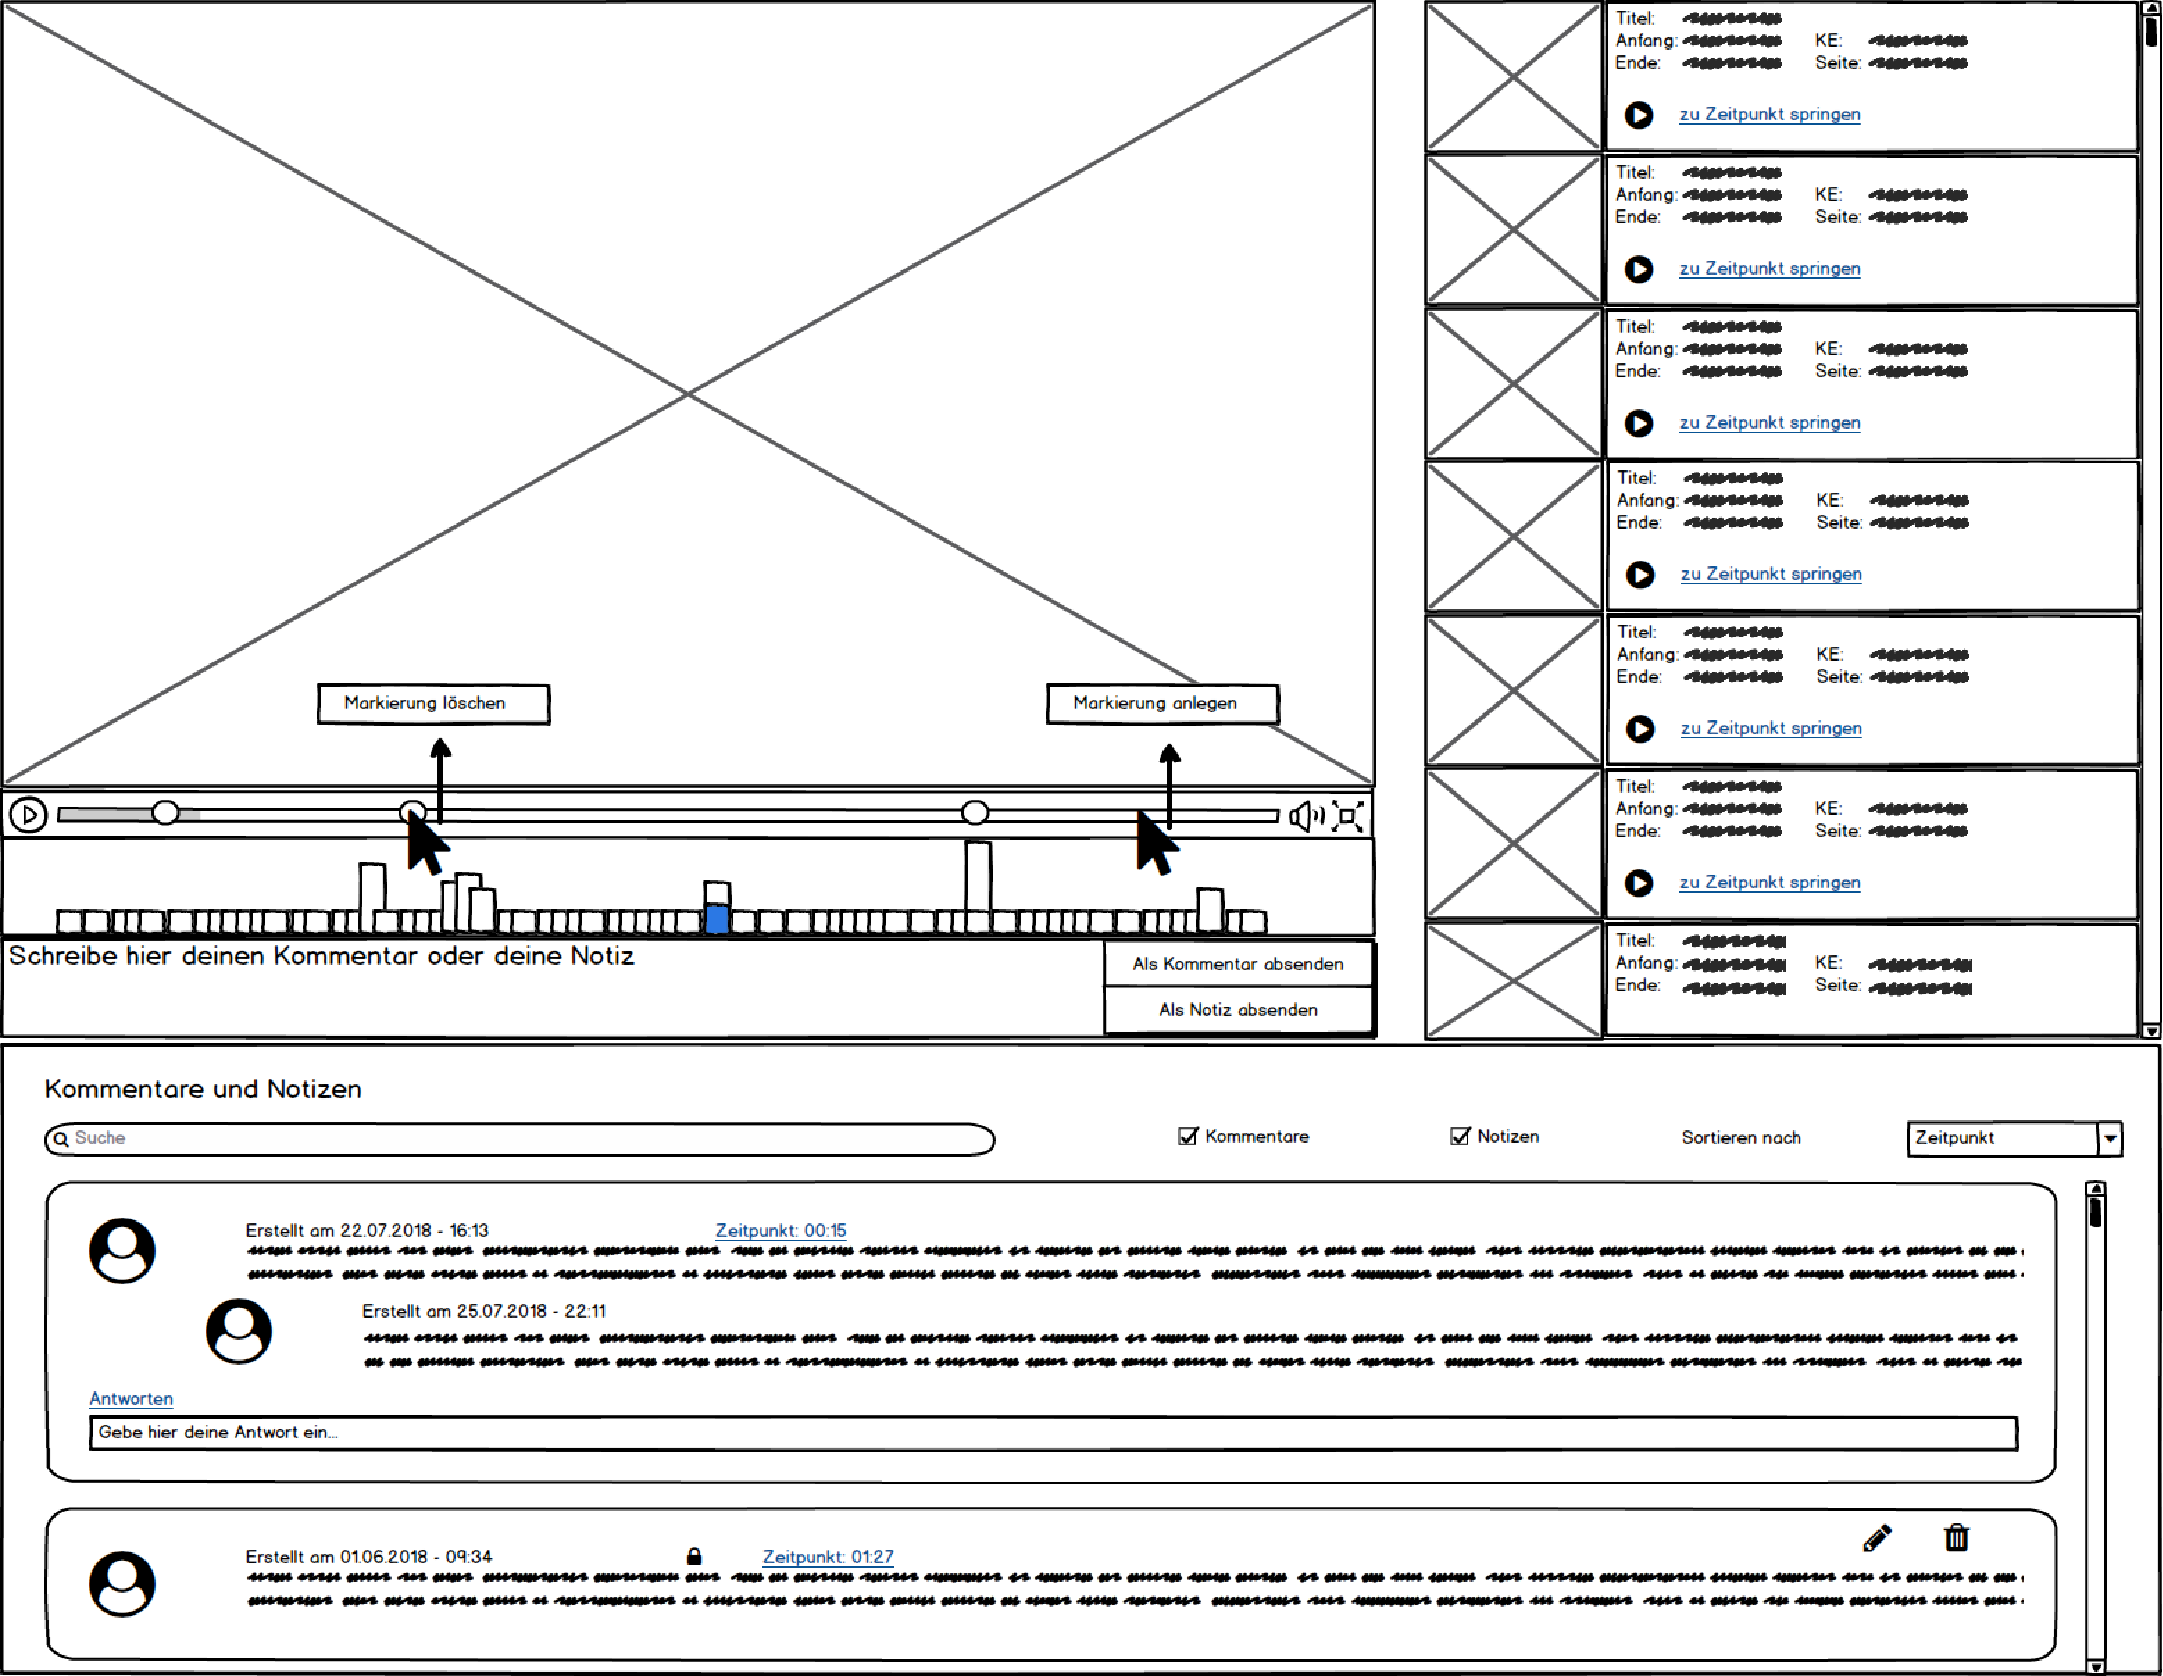
\includegraphics[width=\textwidth,center]{MockupSeiteLayoutVersion1.pdf}
%\caption{\label{fig:MockupSeiteLayoutVersion1}Erstes Layout der Seite für Hyperaudio-Dokumente}
%\end{figure}

%\begin{figure}[h!]
%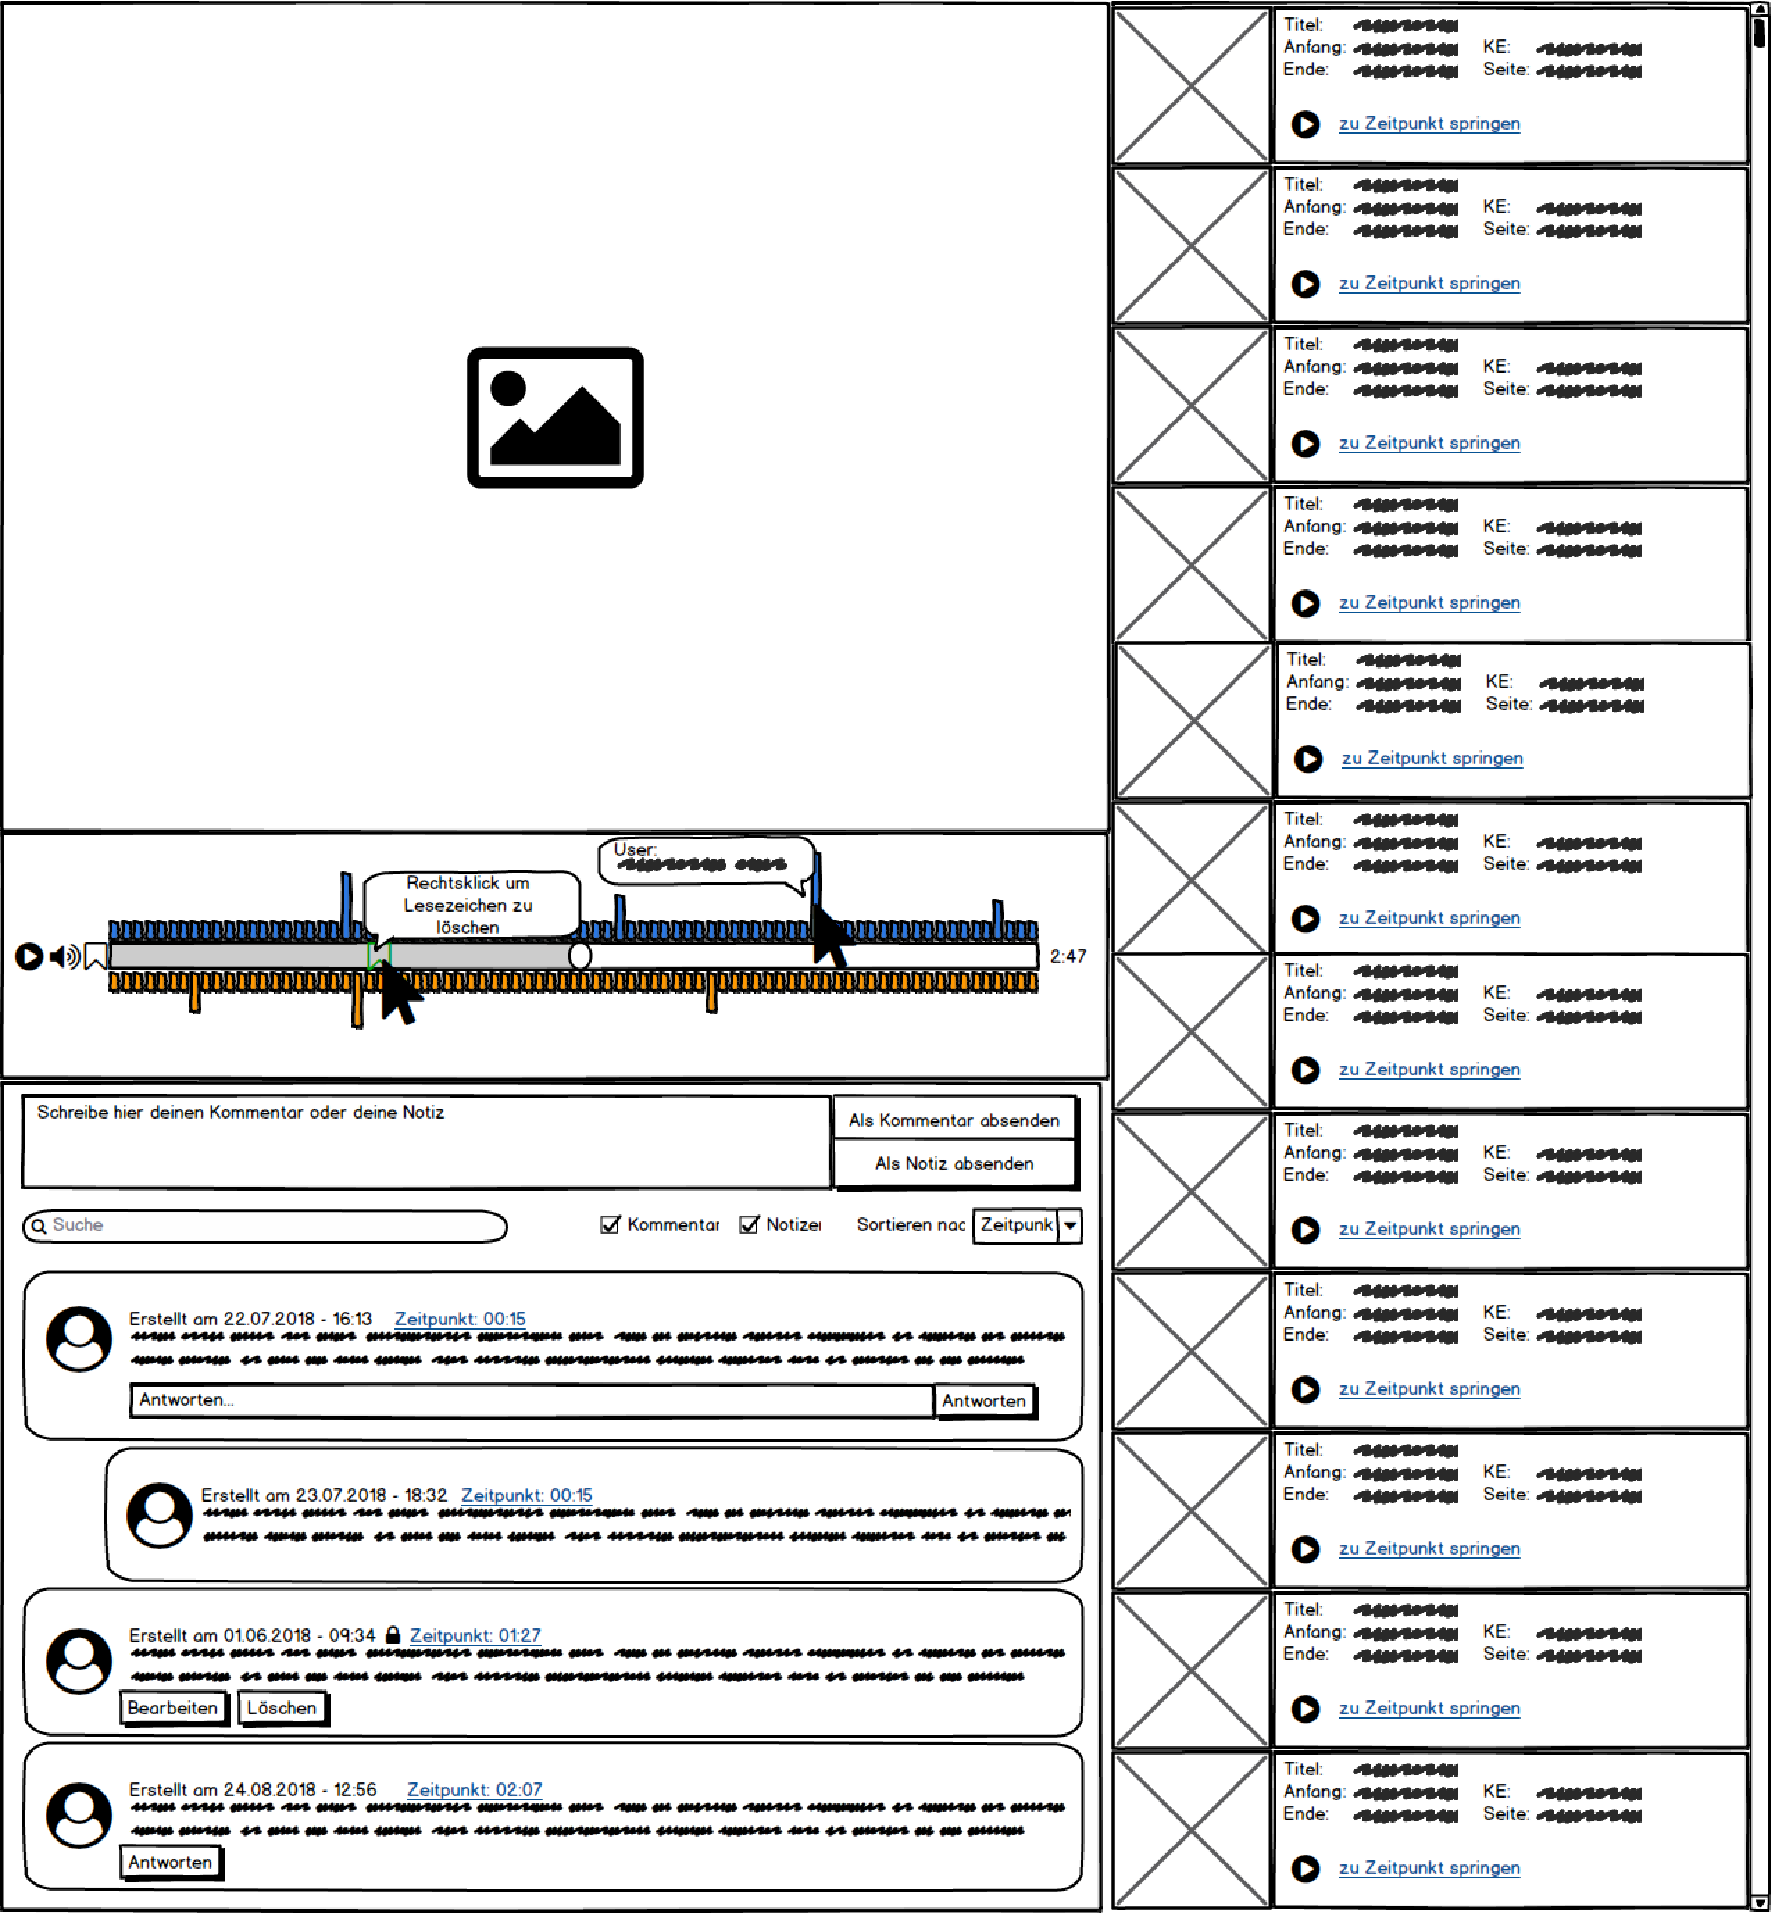
\includegraphics[width=\textwidth,center]{MockupSeiteLayoutFinal.pdf}
%\caption{\label{fig:MockupSeiteLayoutFinal}Finales Layout der Seite für Hyperaudio-Dokumente}
%\end{figure}

\begin{figure}[h!]
\begin{subfigure}[c]{\textwidth}
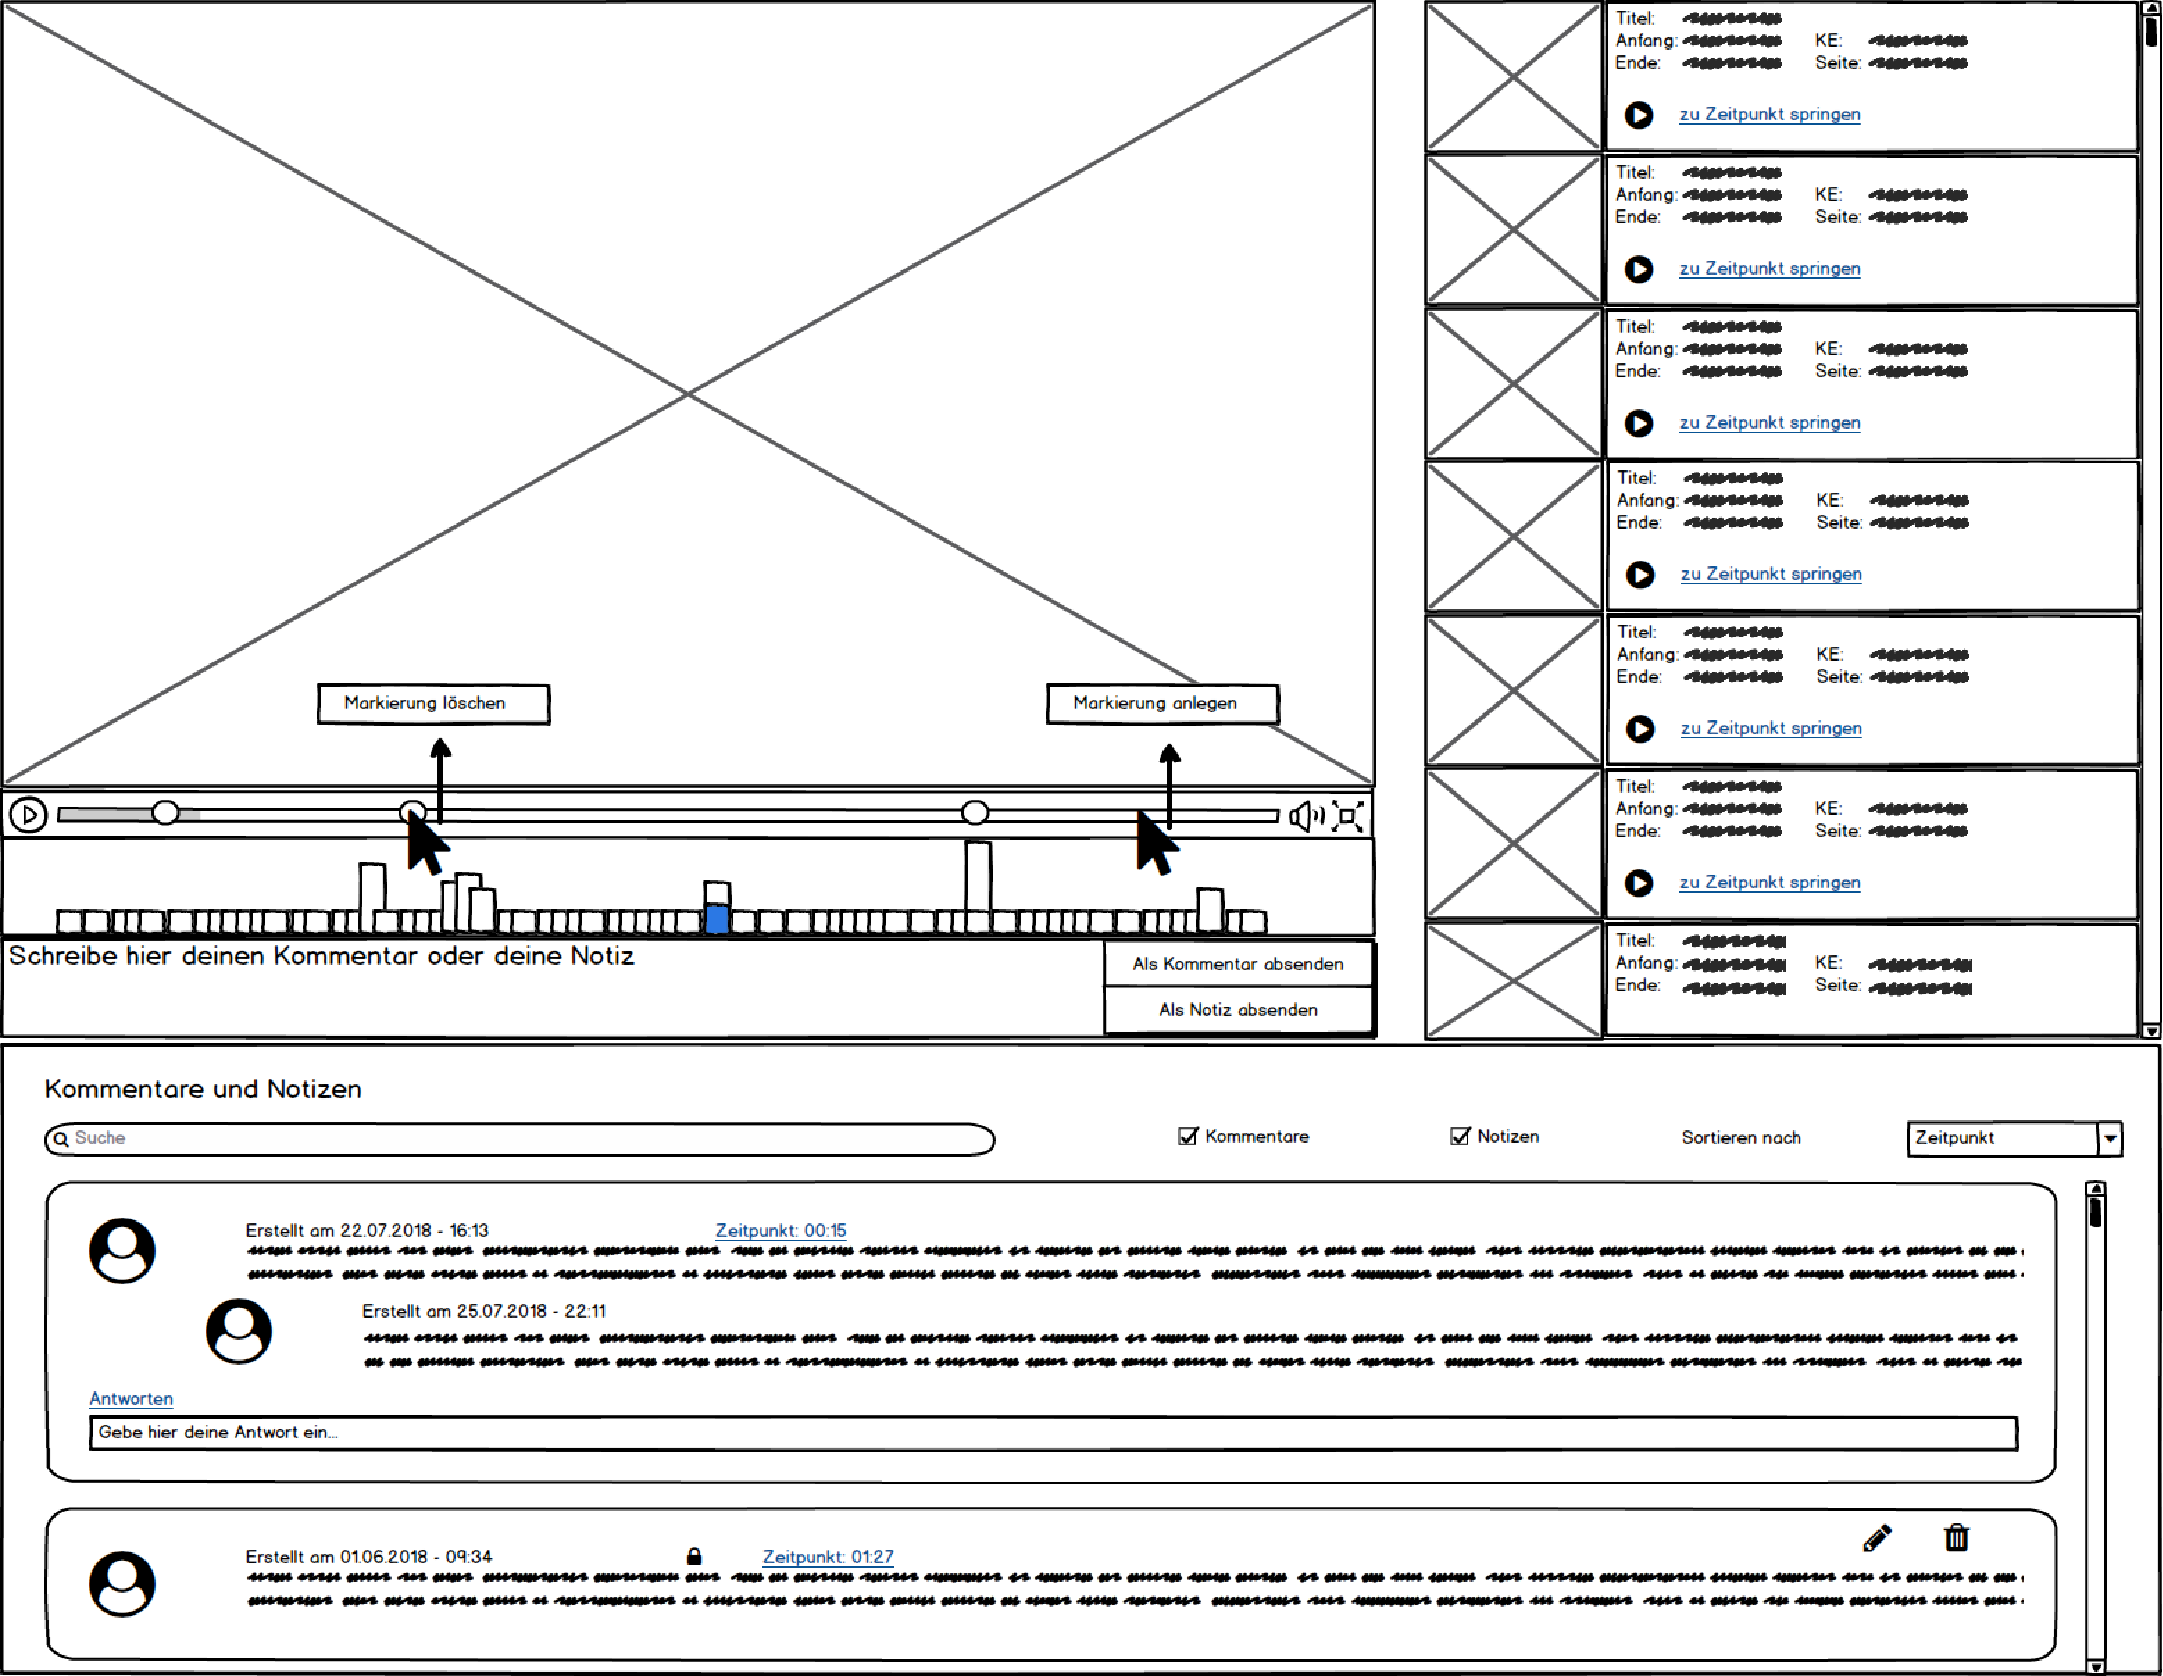
\includegraphics[width=0.9\textwidth,center]{MockupSeiteLayoutVersion1.pdf}
\subcaption{Erste Version}
\label{fig:MockupSeiteLayoutVersion1}
\end{subfigure}
\par\bigskip
\begin{subfigure}[c]{\textwidth}
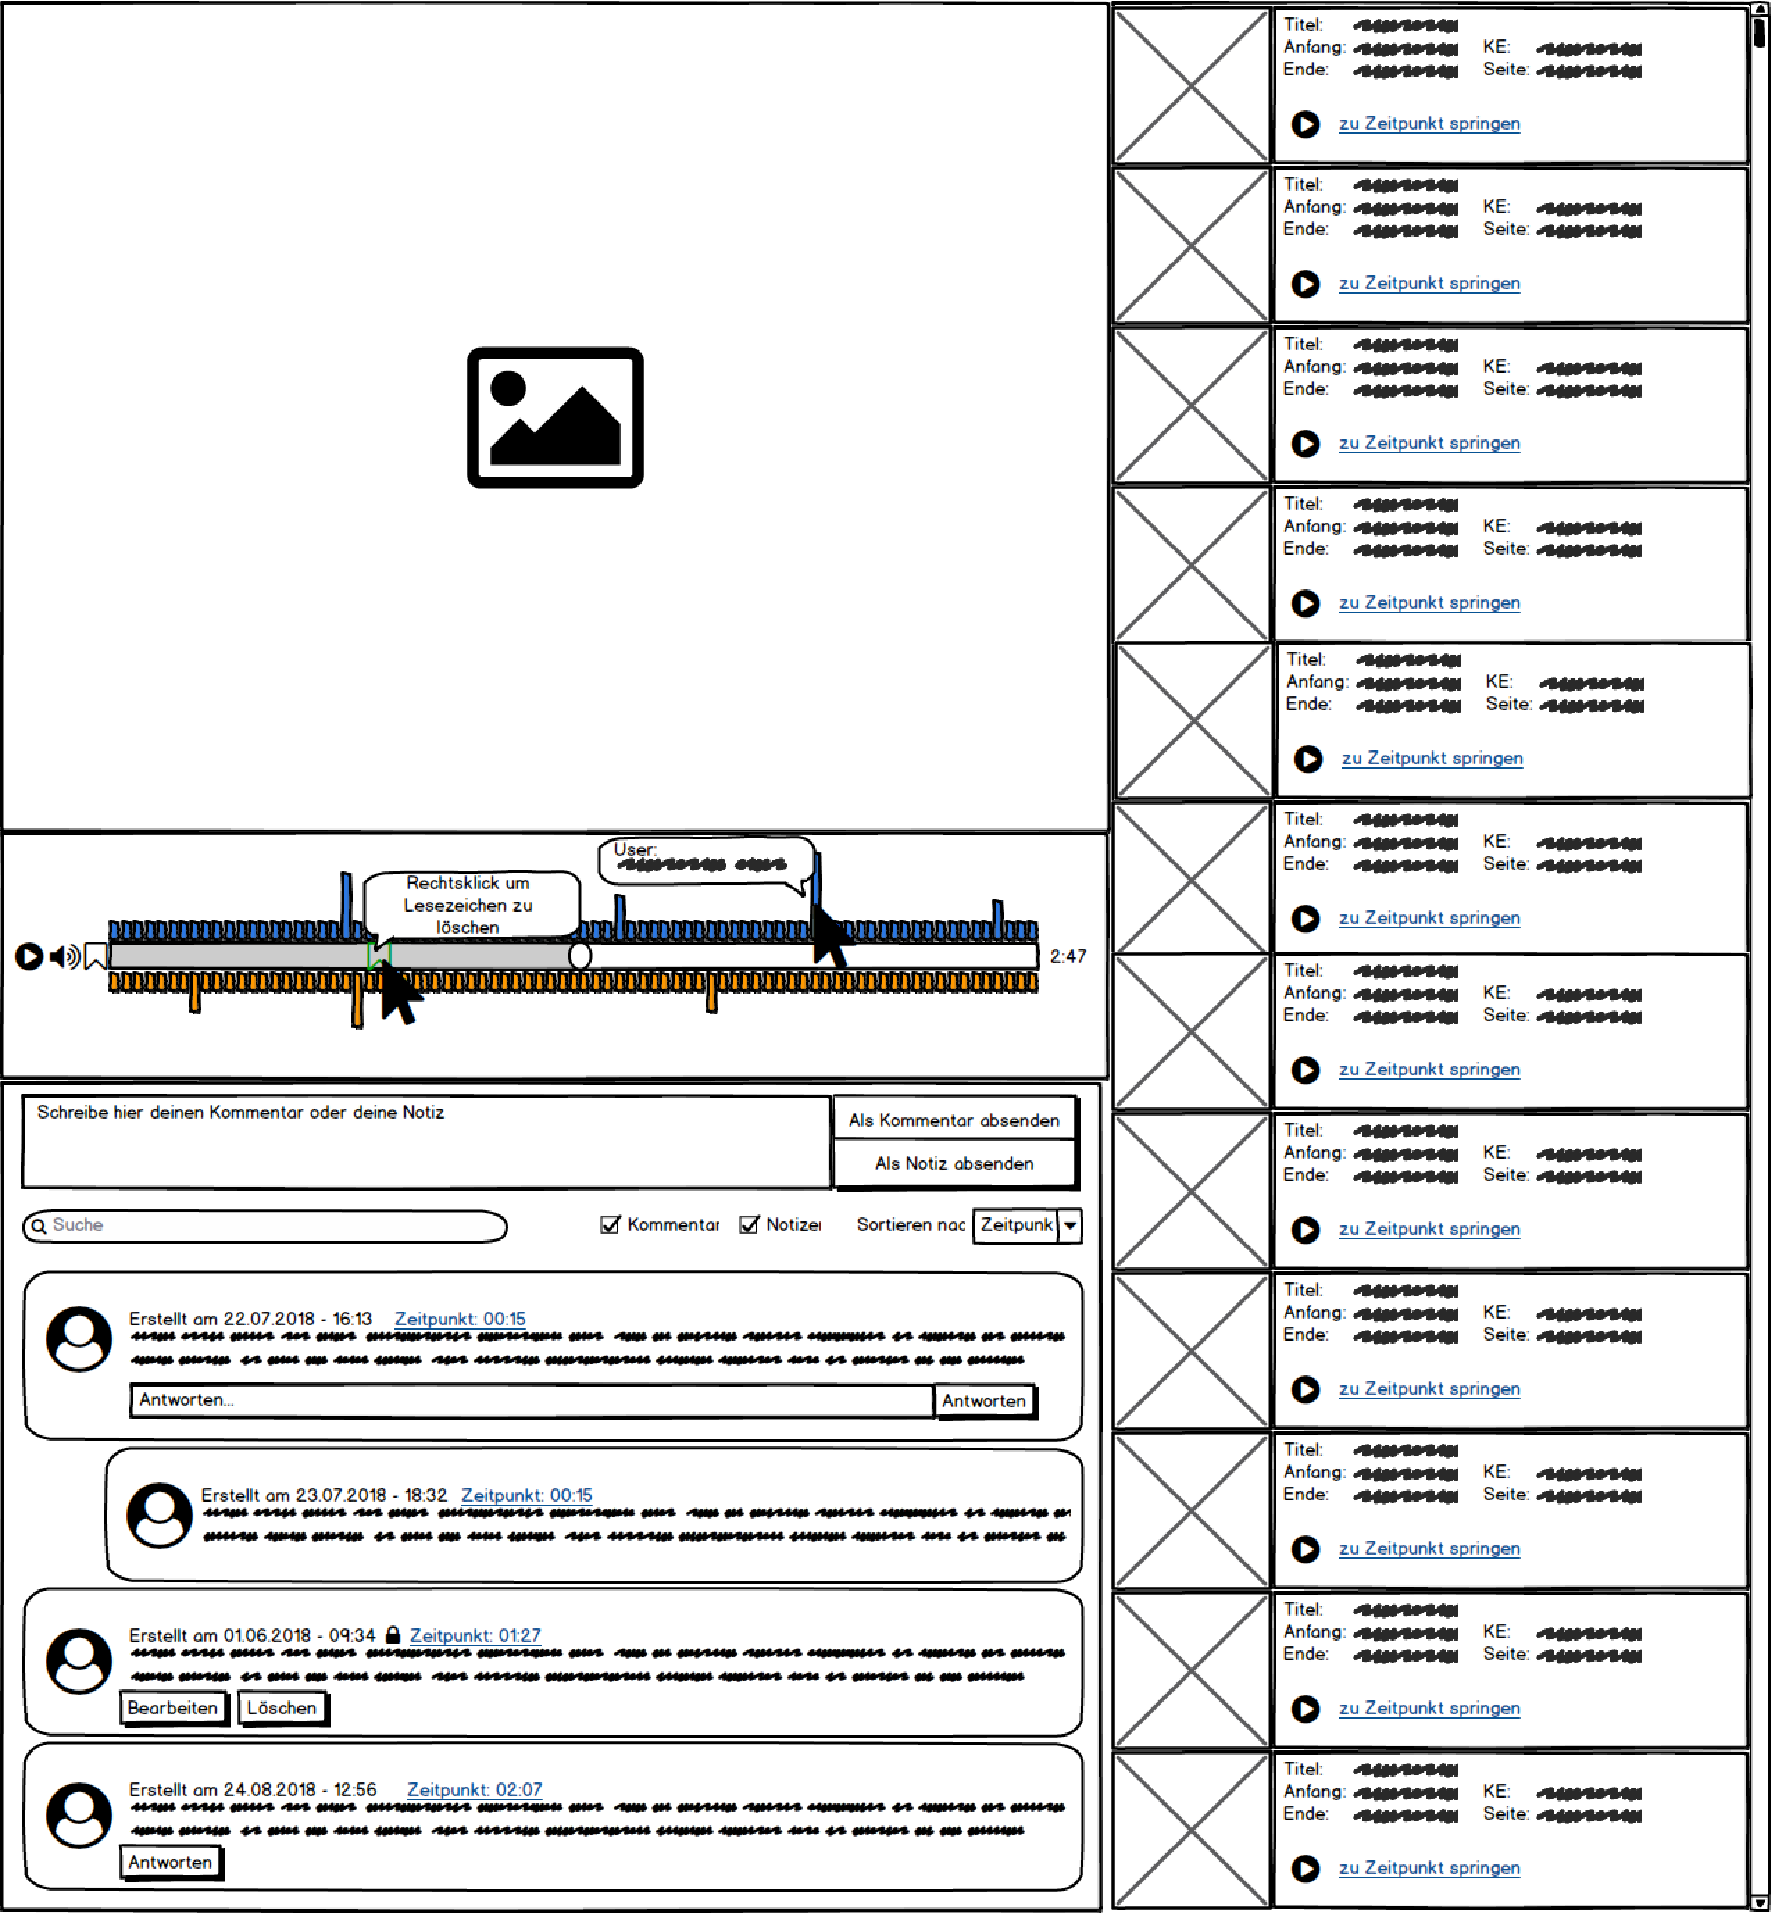
\includegraphics[width=0.9\textwidth,center]{MockupSeiteLayoutFinal.pdf}
\subcaption{Finale Version}
\label{fig:MockupSeiteLayoutFinal}
\end{subfigure}
\caption{Benutzeroberfläche - Layout der Seite für Hyperaudio-Dokumente}
\label{fig:MockupSeiteLayout}
\end{figure}

%%%%%%%%%%
%\subsection{Administrationsseite eines Hyperaudio-Dokuments}
%\dots


%%%%%%%%%%
%\subsection{Moodle-Oberfläche im Allgemeinen}
%\dots








%%%%%%%%%%
\section{Zusammenfassung}
\dots
